% LLNCS macro package for Springer Computer Science proceedings;
% Version 2.21 of 2022/01/12

%%%%%%%%%%%%%%%%%%%%%%%%%%%%%%%%%%%%%%%%%%%%%%%%%
%%%%       FORMATTING OPTIONS AND IMPORTS    %%%%
%%%%%%%%%%%%%%%%%%%%%%%%%%%%%%%%%%%%%%%%%%%%%%%%%

%%%% this docu is oriented for llncs class, 
\documentclass[runningheads]{llncs}
%%%% but other classes might be used 
%\documentclass{article}



\usepackage[T1]{fontenc} 
% T1 fonts will be used to generate the final print and online PDFs,
% so please use T1 fonts in your manuscript whenever possible.
% Other font encondings may result in incorrect characters.

\usepackage{graphicx}
% Used for displaying a sample figure. 
% If possible, figure files should be included in EPS format.

% If you use the hyperref package, please uncomment the following two lines
% to display URLs in blue roman font according to Springer's eBook style:
%\usepackage{color}
%\renewcommand\UrlFont{\color{blue}\rmfamily}
%\urlstyle{rm}

\usepackage{minted}
% To highlight programming languages code 

\usepackage{amsmath,amssymb}

\usepackage{xcolor}
\definecolor{verylightgray}{rgb}{0.97, 0.97, 0.97}

\usepackage{xspace}
\usepackage{ifthen}
\usepackage{hyperref}


%%%%%%%%%%%%%%%%%%%%%%%%%%%%%%%%%%%%%%%%%%%%%%%%%
%%%%            COMMENTS OPTIONS             %%%%
%%%%%%%%%%%%%%%%%%%%%%%%%%%%%%%%%%%%%%%%%%%%%%%%%

\newboolean{showcomments}
%%%%%%% ---> set true or false to show or hide comments
\setboolean{showcomments}{true} 
\ifthenelse{\boolean{showcomments}}
{\newcommand{\nbnote}[3]{
  \fcolorbox{gray}{yellow}{\bfseries\sffamily\scriptsize#1}
  {\color{#2} \sffamily\small$\blacktriangleright$\textit{#3}$\blacktriangleleft$}
  }
}
{\newcommand{\nbnote}[3]{}
 \newcommand{\version}{}
}
%%%%%%% ---> create reviewers' names and colors to show on comments
\newcommand{\fabio}[1]{\nbnote{fabio}{red}{#1}}
\newcommand{\joao}[1]{\nbnote{joao}{blue}{#1}}
\newcommand{\francisco}[1]{\nbnote{francisco}{magenta}{#1}}
% in the text comment like: \francisco{my commment}






%%%%%%%%%%%%%%%%%%%%%%%%%%%%%%%%%%%%%%%%%%%%%%%%%
%%%%               TITLE                  %%%%
%%%%%%%%%%%%%%%%%%%%%%%%%%%%%%%%%%%%%%%%%%%%%%%%%

\begin{document}

\title{Reentry Simulation}

\author{João Garção (Nº 62663) \and\\ Fábio Silva (Nº 62730) \and \\Francisco Silva (Nº 63585)}

\authorrunning{ }
%%%% ---> Write the author name to appear in the page headers
% First names are abbreviated
% If there are more than two authors use 'et al.' 



\institute{NOVA School of Science and Technology}
% if multiple institutes, use \and to separate each one: \institute{Princeton University \and Springer Heidelberg} and in authors identify the institute of each author: ex AuthorA\inst{1,2} and AuthorB{2}


\maketitle      % typeset the header of the contribution


%%%%%%%%%%%%%%%%%%%%%%%%%%%%%%%%%%%%%%%%%%%%%%%%%
%%%%               ABSTRACT                  %%%%
%%%%%%%%%%%%%%%%%%%%%%%%%%%%%%%%%%%%%%%%%%%%%%%%%

\begin{abstract}
Simulating complex physical phenomena is a crucial step in various fields, including science, industry, research and development. However, these simulations often demand significant computational resources, making it essential to leverage specialized software and libraries. How do we determine the necessary precision against the available computational power and time? How can we find the right balance? What are the different methods and their respective advantages and disadvantages? This paper addresses these questions through the lens of simulating the cinematic reentry of a capsule into Earth's atmosphere. We explore the forces of gravity, drag, and lift, along with the deployment of a parachute before landing. This research, part of the Computational Modelling and Simulation in Engineering Physics discipline, represents a step forward in our ongoing effort to master and implement diverse simulation methodologies and techniques.


\keywords{Physics \and Simulation \and Cinematic \and Reentry}

\end{abstract}




%%%%%%%%%%%%%%%%%%%%%%%%%%%%%%%%%%%%%%%%%%%%%%%%%
%%%%               INTRODUCTION              %%%%
%%%%%%%%%%%%%%%%%%%%%%%%%%%%%%%%%%%%%%%%%%%%%%%%%

\section{Introduction}
% Context and Motivation
The discipline of Computational Modelling and Simulation in Physics Engineering equips students and researchers with the essential tools and techniques to develop sophisticated simulations. This field is pivotal in achieving accurate and reliable results while efficiently managing computational resources. As simulations become increasingly complex, striking the right balance between precision and computational power is crucial. This discipline not only imparts the technical skills required but also fosters a deep understanding of how to optimize simulations for the best performance, making it an indispensable area of study for tackling real-world engineering challenges.

% Research Goals
This research focuses on simulating the reentry of a capsule into Earth's atmosphere, aiming to determine the optimal reentry parameters. The goal is to ensure the trajectory stays within specified constraints, such as minimizing maximum acceleration during descent, controlling landing velocity, and achieving a precise landing range. By fine-tuning these parameters, we aim to enhance the safety and reliability of the reentry process, providing valuable insights for future aerospace missions.

% Contributions
In this paper, we introduce a tool available on GitHub \cite{git} that simulates the reentry of a capsule into Earth's atmosphere. Starting from an initial altitude of 130 000 meters, users can set the initial angle and velocity as the capsule descends under the influence of gravity, drag, and lift forces. The simulation also accounts for the deployment of a parachute at lower altitudes and velocities. The tool offers configurable parameters and various simulation modes, such as normal descent, orbital velocity, or escape velocity scenarios. Additionally, it allows for choosing between a flat Earth or a round Earth model, with lift forces oriented either perpendicular to gravity or to the velocity vector. The paper includes a set of plots to illustrate the simulation results, facilitating easier analysis of the reentry phenomenon.

% Paper structure
This paper is organized as follows:

-\textbf{Section 2}: Provides an overview of the developed application, including its structure, a basic user guide, and instructions on how to run the intended simulations with different parameters and profiles.

- \textbf{Section 3}: Presents the fundamental physics concepts essential for understanding the simulations. This section also describes the assumptions and model simplifications considered.

- \textbf{Section 4}: Explains the various mathematical methods used to calculate the simulations implemented in the program, including the forward Euler method, the implicit method, and the Runge-Kutta method employed by the `solve\_ivp` Python module.

- \textbf{Section 5}: Discusses the simulation results, highlighting key observations and findings.

- \textbf{Section 6}: Concludes the paper with a summary of the conclusions drawn from the study.



%%%%%%%%%%%%%%%%%%%%%%%%%%%%%%%%%%%%%%%%%%%%%%%%%
%%%%             APPLICATION                 %%%%
%%%%%%%%%%%%%%%%%%%%%%%%%%%%%%%%%%%%%%%%%%%%%%%%%

\section{Application Structure and User Manual}
In this section, we will provide a brief overview of the application we developed to contextualize the subsequent analysis. Additionally, we aim to offer users a straightforward guide on how to use the app and explore its various capabilities.

\subsection{Code Structure}
The developed application \cite{git} is organized into multiple Python scripts, as illustrated in Fig~\ref{app_structure}.

\begin{figure}
\centering
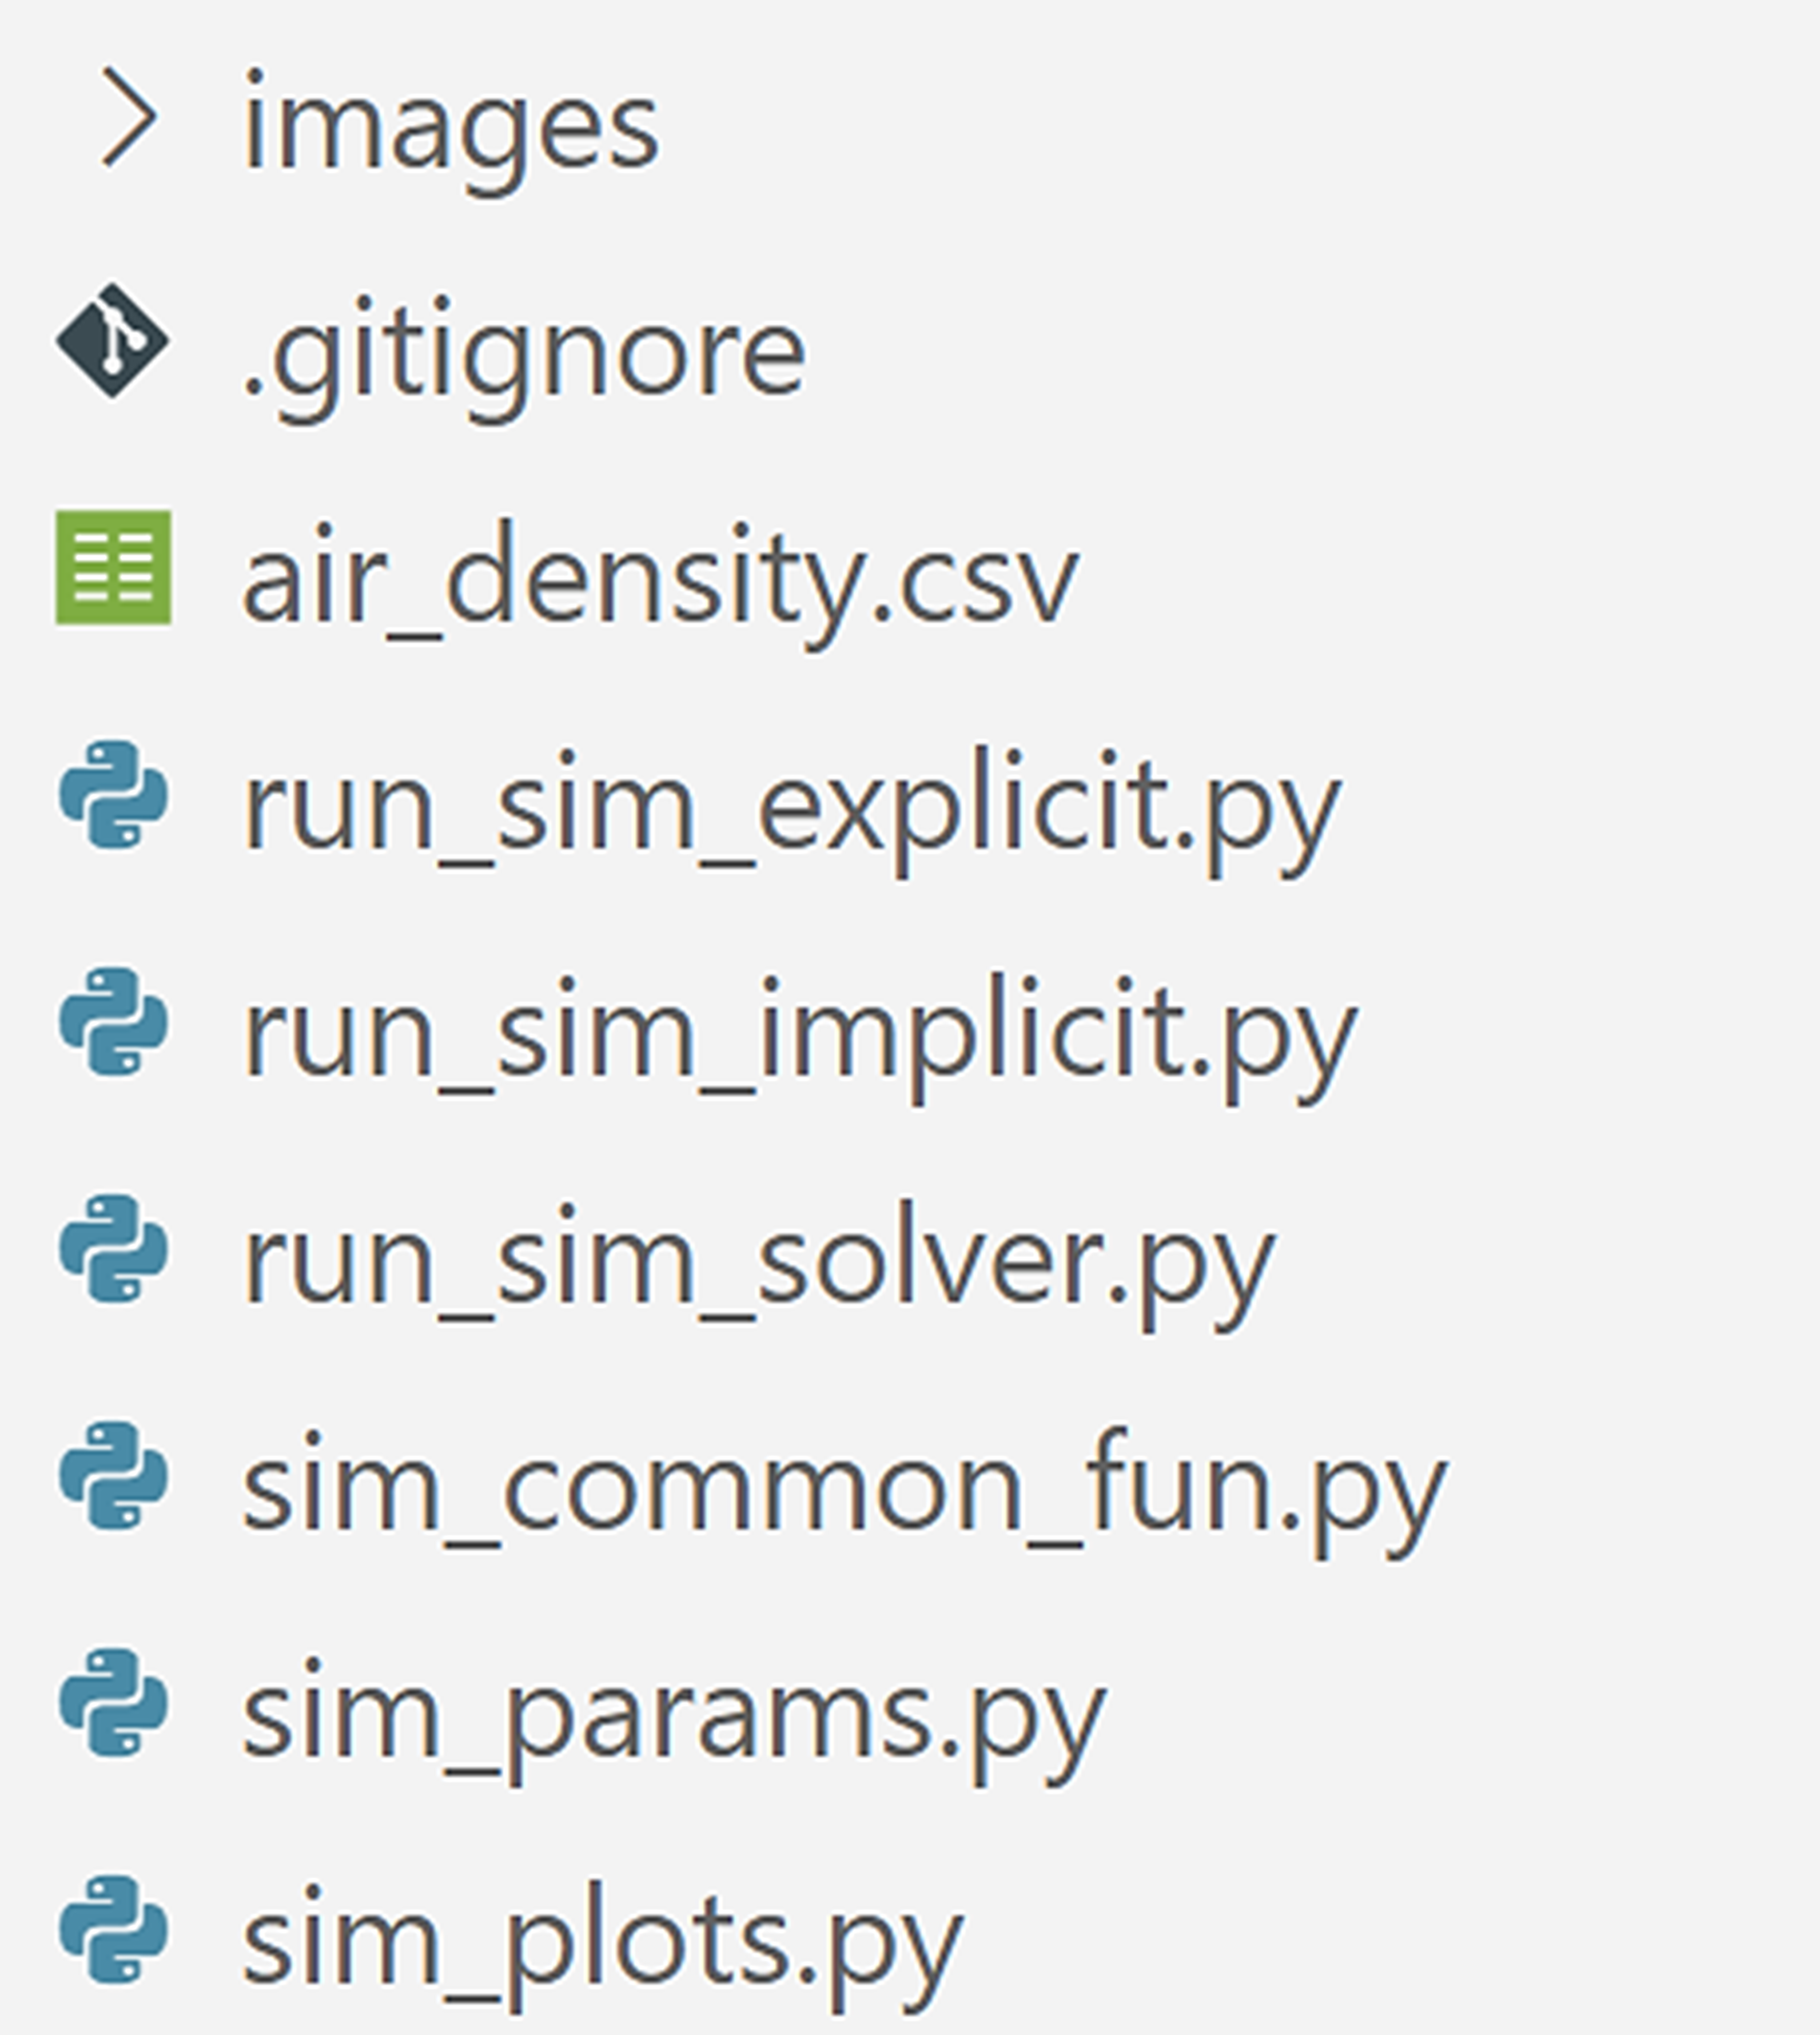
\includegraphics[width=0.4\textwidth]{images/app_structure.png}
\caption{App Structure \cite{git}} \label{app_structure}
\end{figure}






\subsection{App Usage}

%%%%%%%%%%% SIM_PARAMS

\textbf{Selection of Simulation Parameters:\\}
Within the document sim\_params, users can configure various simulation options.

\begin{minted}[frame=lines, bgcolor=verylightgray, fontsize=\small, linenos, numbersep=1pt]{python}
''' 1. Choose if you want to save plot images in the folder "images". '''
SAVE_PLOT_IMAGES = False
SIM_NAME_FOR_IMAGE = "image_name" 


''' 1. Choose the simulation to run from the options below '''
SIM_TO_RUN = 2
# --------------------------------------------------------------------
# REENTRY_SIMULATION OPTIONS: 
REENTRY_SIM_NORMAL = 1                  # multiple init angles and vel
REENTRY_SIM_CUSTOMIZED_PAIRS = 2        # with chosen angles and vel
REENTRY_SIM_VERTICAL_MOV = 3            # without velocity 
REENTRY_SIM_HORIZONTAL_MOV = 4          # with no forces
REENTRY_SIM_ORBITAL_MOV = 5             # with orbital velocity 
REENTRY_SIM_ESCAPE_VEL_MOV = 6          # with escape velocity 
# PROJECTILE_SIMULATION OPTIONS: 
PROJECTILE_SIM = 7                      # projectile simulation
# --------------------------------------------------------------------

''' 2. Choose more options: '''

# Pairs to run in REENTRY_SIM_CUSTOMIZED_PAIRS
INIT_ANGLES = [-1, -2, -4, -8] # initial angles (degrees)
INIT_VELOCITIES = [2_000, 4_000, 8_000] # initial velocities (m/s)

SIM_WITH_PARACHUTE = True          # Open parachute when met conditions

LIFT_PERPENDICULAR_TO_VELOCITY = False  # 90º to gravity or velocity

MAX_ANGLE_OF_ATTACK = 0                 # to adjust for max lift 

ROUND_EARTH = False                  # flat vs round earth

...
\end{minted}

\noindent\textbf{Executable Simulation Scripts:\\}
After selecting the simulation parameters in the previous script, users should run the simulation using the corresponding method or technique-specific document. The scripts run\_sim\_explicit, run\_sim\_implicit, and run\_sim\_solver are tailored to execute the simulation using distinct methods: explicit Euler, implicit Euler with the Newton method for root finding, and a solver (solve\_ivp from the Python library scipy.integrate), respectively. The solver automates the solution of the system of ordinary differential equations (ODEs) using the default Explicit Runge-Kutta method (RK45).

\noindent \textbf{\\Helper Scripts\\}
Each simulation execution script utilizes essential functions, including derivative calculation, slope determination for the model, and methods for executing simulations across all specified pairs of angles and velocities. These functions are implemented in the document sim\_common\_fun.

Additionally, after completing each set of simulations, results are visualized through various metrics and simulation conditions. These plots are defined in the document sim\_plots.

\noindent \textbf{\\Running the Simulation\\}
To execute the previously presented executables, such as in VS Code, simply open the respective document and click the "Run" button. Alternatively, to run in a terminal, navigate to the directory containing the file reentry\_app.py (cd <path>) and execute the command, for example, python run\_sim\_explicit.py.

The first time you run the program, errors may occur if the necessary libraries are not installed on your computer. In such cases, you will need to install them using commands like:

\begin{minted}[frame=lines, bgcolor=verylightgray, fontsize=\small, linenos, numbersep=1pt]{console}
pip install numpy
pip install scipy
...
\end{minted}

When tests include plots, it is necessary to close each plot before the next one is displayed.












%%%%%%%%%%%%%%%%%%%%%%%%%%%%%%%%%%%%%%%%%%%%%%%%%
%%%%               PHYSICS OF SIMULATION                  %%%%
%%%%%%%%%%%%%%%%%%%%%%%%%%%%%%%%%%%%%%%%%%%%%%%%%
% To easy go to sections use the left 

\section{Physics of Simulation}
In this section, we introduce the fundamental concepts and physical laws that underpin our model and simulation. We also outline the assumptions made in our simulation, acknowledging the practical constraints that prevent consideration of every criterion. Our simulation is based on the model depicted in Fig. \ref{model_forces}, which illustrates the forces incorporated: gravity ($mg$), drag ($D$), and lift ($L$). Additionally, it outlines how the round Earth model influences the reference system used for calculations, where $R$ represents the radius of Earth and $r$ is the radius of Earth plus the altitude above Earth's surface. $\theta$ is the angle from the y-axis to the current position, and $v$ is the velocity.



\begin{figure}
\centering
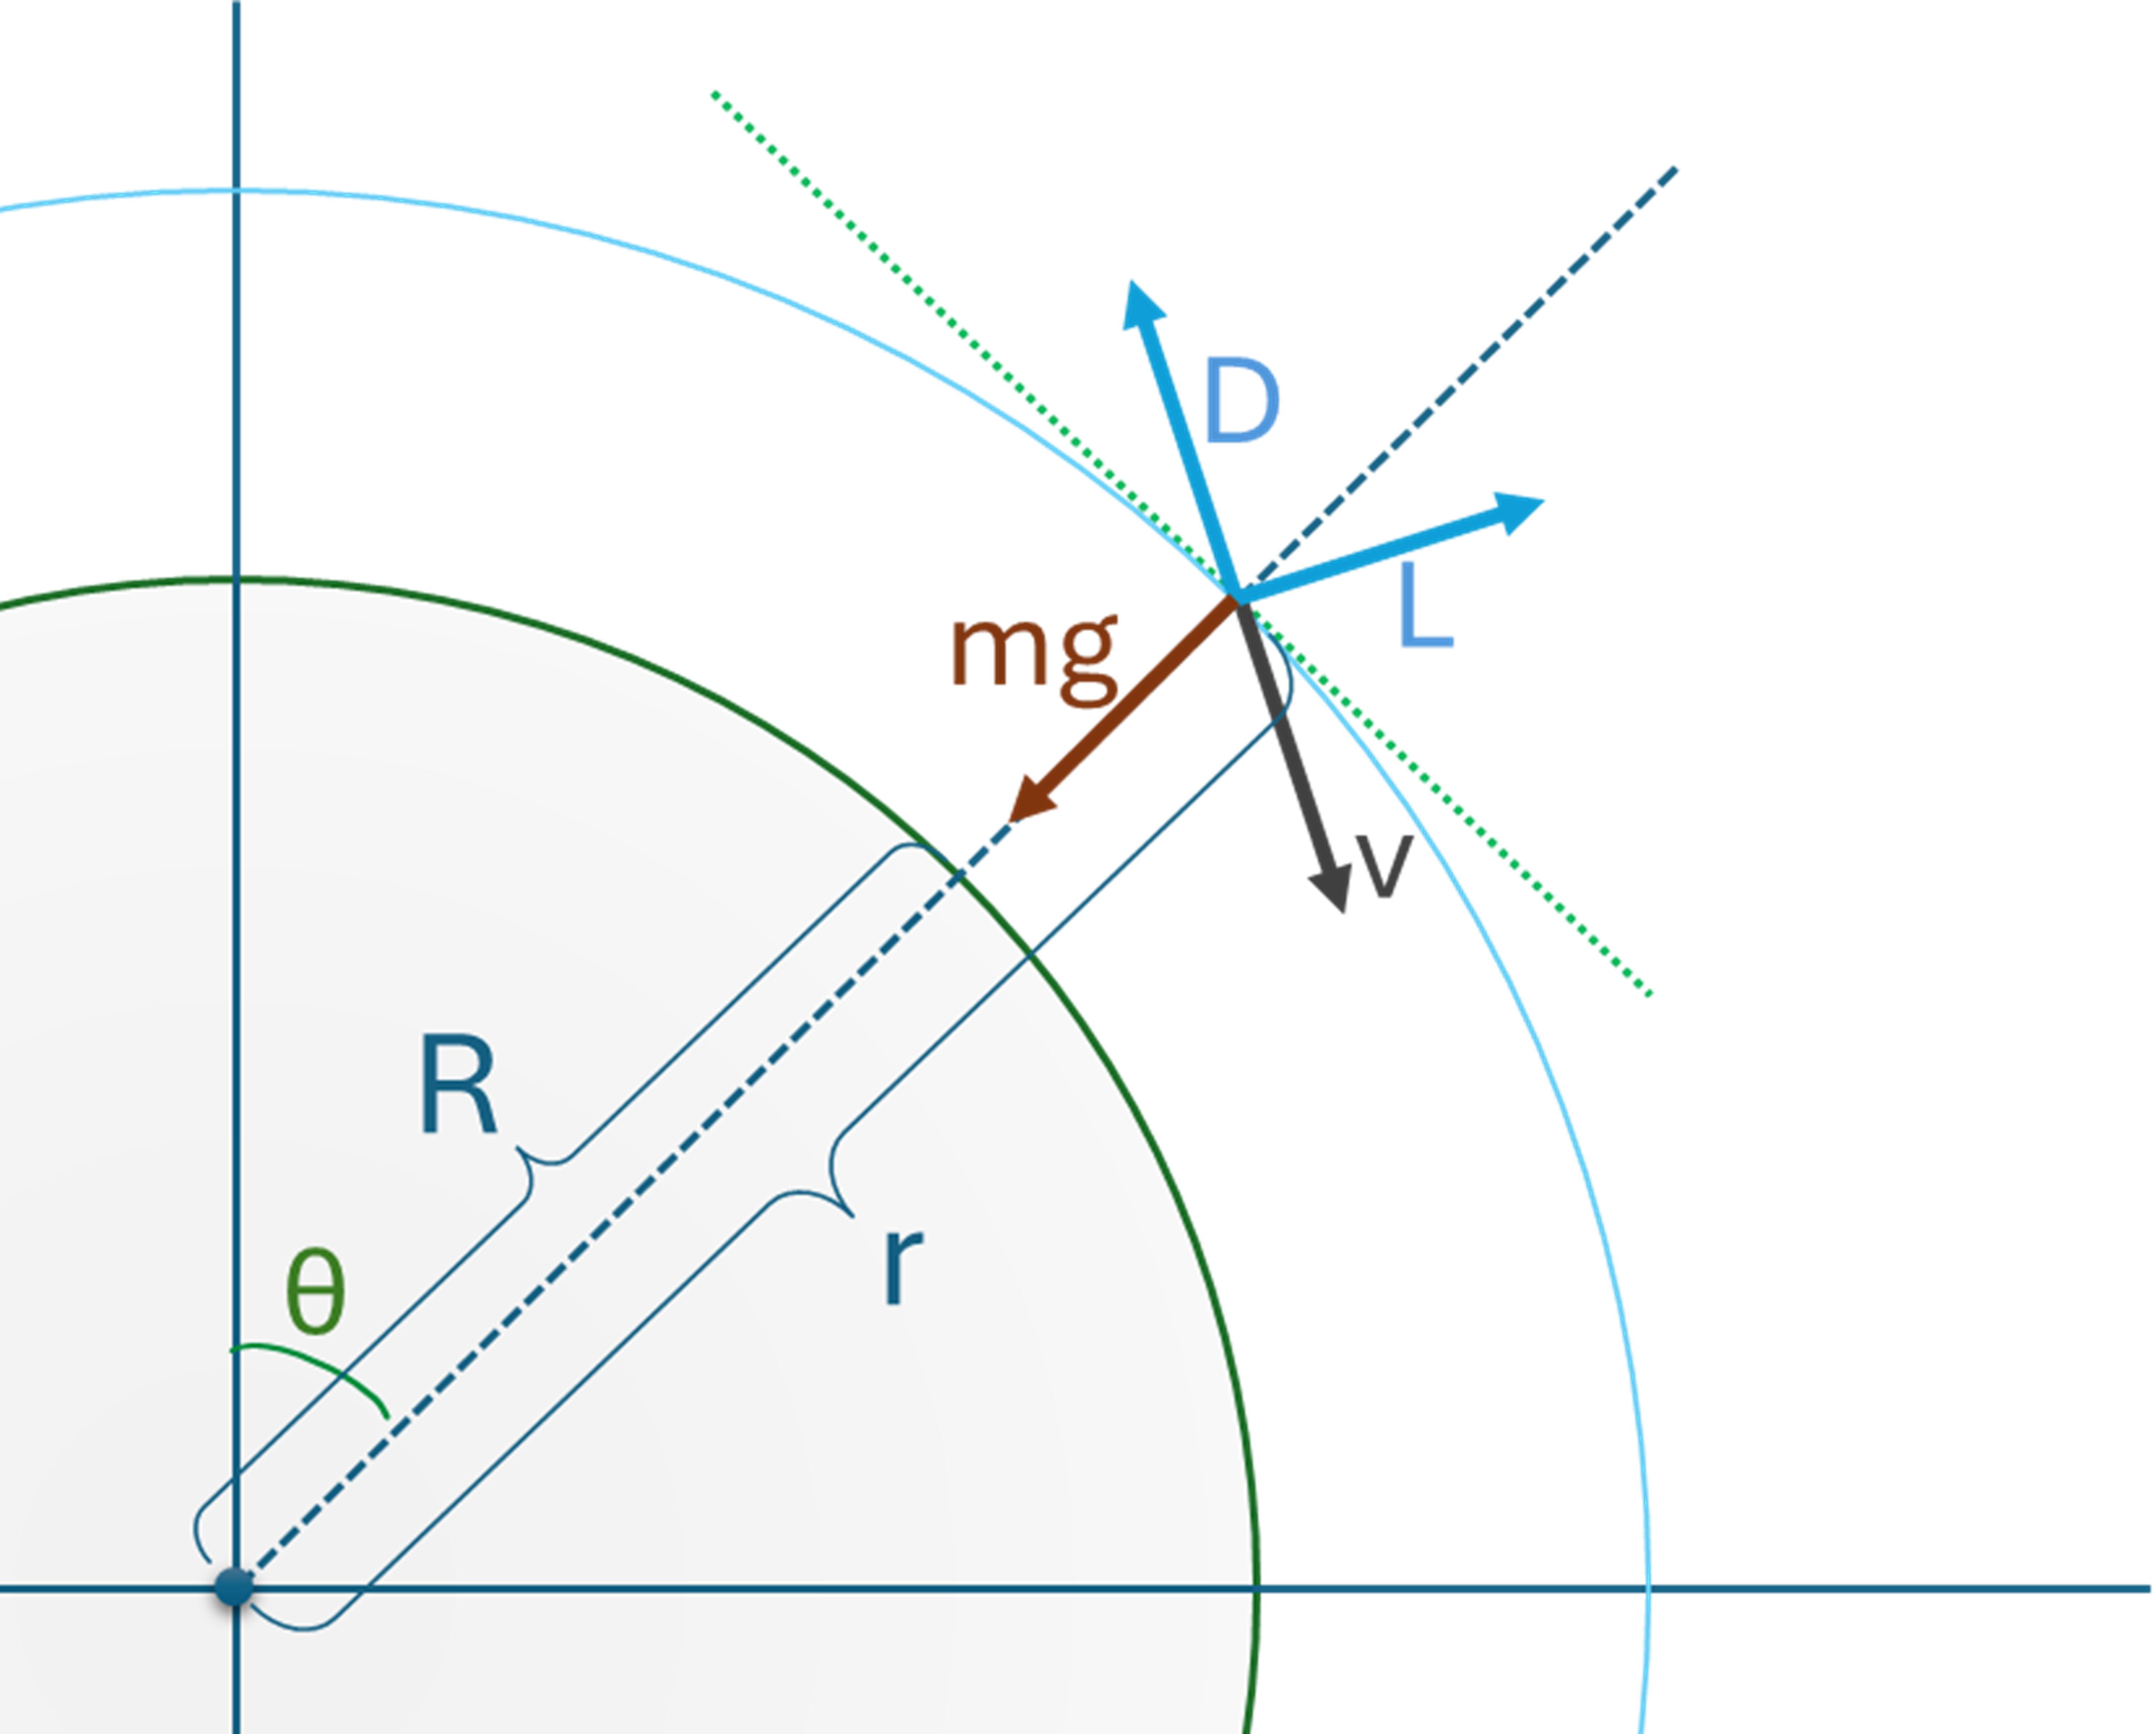
\includegraphics[width=0.65\textwidth]{images/model_forces.png}
\caption{Model Forces} \label{model_forces}
\end{figure}


%%%%%%%%%%%%%%%%%%      GRAVITY     %%%%%%%%%%%%%%%%%%%%%%

\subsection{Gravity}
At the core of this simulation lies the gravitational force, essential for understanding the dynamics of objects in Earth's atmosphere. Unlike simpler simulations, the force of gravity varies with altitude from the Earth's surface, calculated relative to the center of the Earth. By default, gravitational force is computed using Newton's Law of Universal Gravitation, adjusting according to the distance between two objects—in this case, the Earth's center and the capsule or the projectile. The gravitational force \textbf{\( F_G \)} is defined by the following formula, where \textbf{M} and \textbf{m} are the masses of the Earth and the object in kilograms, \textbf{r} is the distance between the Earth's center and the object in meter\cite{orlando_trajectory}s:

\begin{equation}
F_G = \frac{G \cdot M \cdot m}{r^2}
\end{equation}
Here, \( G \) is the gravitational constant with a value of \( 6.67430 \times 10^{-11} \) N⋅(m²/kg²).

In simulations, our goal is to evaluate the position, velocity, and acceleration of the object. For this purpose, we apply Newton's second law, which states:
\begin{equation}
F_G = ma
\end{equation}
where \textbf{m} is the mass of the object in kilograms, and \textbf{a} is the acceleration in m/s². Solving for \textbf{a} gives us the acceleration, which we then integrate to obtain velocity and further integrate to determine position.
Thus, the acceleration due to gravity  is:
\begin{equation}
a_x = 0 \quad \text{and} \quad a_y = \frac{G \cdot M}{r^2}
\end{equation}

This gravitational force acts solely on the y-component, causing a reduction in altitude. Therefore, we subtract the acceleration due to gravity from the object's total acceleration in the y-component:

\begin{minted}[frame=lines, bgcolor=verylightgray, fontsize=\small, linenos, numbersep=1pt]{console}
ay -= g
\end{minted}

Understanding these gravitational principles is crucial for accurately modeling the descent of objects through Earth's atmosphere in our simulation.



%%%%%%%%%%%%%%%%%%      DRAG     %%%%%%%%%%%%%%%%%%%%%%

\subsection{Drag}
The simulation also accounts for the drag force, which significantly affects the motion of objects in Earth's atmosphere. Unlike gravitational force, which diminishes with altitude, drag force increases with an object's speed and encounters resistance from the surrounding air. This force opposes the direction of the object's motion, reducing its speed over time.

The drag force \( F_D \) is calculated using the following formula, where \( \rho \) represents the air density, \( A \) is the cross-sectional area of the object facing the direction of motion, and \( C_D \) is the drag coefficient that depends on the shape and surface roughness of the object \cite{gallais_mechanics}:

\begin{equation}
F_D = \frac{1}{2} \rho A C_D v^2 
\end{equation}

Here,\textbf{v} denotes the velocity of the object relative to the air.

\textbf{\\Drag Acceleration\\}
Similar to gravity, the acceleration due to drag force can be determined using Newton's second law, 
\textbf{F = ma}. However, unlike gravity, which acts vertically downward in full force, drag force opposes the velocity of the object. Therefore, the acceleration components caused by drag in both the \textbf{x} and \textbf{y} directions depend on the velocities in those respective axes.
Thus, we can calculate the acceleration along the x-axis based on the velocity and its \textbf{x} and \textbf{y} components. E.g. for x component \cite{chapman_analysis}:

\begin{equation}
a_x = - \frac{1}{2} \frac{\rho A C_D v^2 \cdot v_x}{v m}
\end{equation}
Here, \textbf{vx} represents the velocity of the object in the \textbf{x} direction. Dividing by \textbf{v} normalizes the velocity to determine the correct amount of the x-component velocity. The negative sign is employed because drag acts in opposition to velocity, thereby reducing its magnitude. Hence, while \( v^2 \) is always positive, each component velocity, such as \textbf{vx}, retains its respective sign. Consequently, the negative sign in the drag acceleration consistently opposes the direction of the velocity. The equation for the 
y-component is similar.

\textbf{\\Simulation of Drag\\}
The default simulation models the reentry of a capsule into Earth's atmosphere using predefined constants, such as its drag coefficient. Additionally, there is an option to deploy a parachute once certain criteria, such as maximum altitude and velocity, are met. In the simulation, when the parachute is deployed, its drag coefficient and acceleration are added to that of the capsule.



%%%%%%%%%%%%%%%%%%      LIFT     %%%%%%%%%%%%%%%%%%%%%%

\subsection{Lift}
Finally, another force to consider is the lift force, which depends on the lift coefficient. This coefficient is influenced by the shape and orientation of the object and determines the magnitude of the lift force. The formula for lift force is analogous to that of drag force, but incorporating a lift coefficient, instead of a drag coefficient \cite{orlando_voxels}:

\begin{equation}
F_L = \frac{1}{2} \rho A C_L v^2
\end{equation}

\textbf{\\Simulation of Lift\\}
In the simulation, we typically apply lift perpendicular to gravity by default. This simplifies the application of the lift force, directing all lift acceleration to the y-component, and increasing it proportionally to velocity. Consequently, when an object descends vertically, gravity pulls downward, while both drag and lift exert an upward force. In other directions of motion, gravity always acts downward (negative sign), lift always acts upward (positive sign), and drag opposes the velocity (negative sign) to decelerate the object. So the lift acceleration, which is entirely applied in the y-axis, can be expressed as \cite{miguel_optimal_reentry_control}:

\begin{equation}
a_x = 0 \quad \text{and} \quad a_y = \frac{1}{2} \frac{\rho A C_D v^2}{m}
\end{equation}


However, a key characteristic of the lift force is its orientation perpendicular to the velocity vector \cite{reentry_matters}. In our simulation, we also have the option to model this lift force as being perpendicular to the velocity. To that end, we start by determining the velocity angle, for example, by calculating the angle from given \( v_x \) and \( v_y \). Subsequently, we determine the lift angle perpendicular to the velocity. One assumption we make is that the capsule is always well-oriented, ensuring that the lift force always acts upwards. This means the object does not rotate, and regardless of its direction of motion, the lift force is considered to act upwards. To enforce this, if the calculated lift angle exceeds \(\pi\), we adjust it accordingly. With the absolute lift value known, we then calculate the acceleration components as follows:

\begin{minted}[frame=lines, bgcolor=verylightgray, fontsize=\small, linenos, numbersep=1pt]{python}
vel_angle = np.arctan2(vy, vx) # Velocity angle
lift_angle = vel_angle + np.pi/2 # Lift angle perpendicular
if lift_angle > np.pi:  # Adjust lift to always be positive   
    lift_angle -= np.pi 
ax = a_lift * np.cos(lift_angle) # Acceleration in x-direction
ay = a_lift * np.sin(lift_angle) # Acceleration in y-direction
\end{minted}


\textbf{\\Angle of Attack\\}
For the reentry simulations, the capsule is initially set to undergo a ballistic reentry without the ability to adjust its trajectory. However, an option was implemented to orient the capsule's angle of attack \footnote{The angle of attack is the angle between the vehicle’s nose and its velocity vector \cite{returning_space}.}, allowing us to optimize the use of lift for a smoother descent. In the default simulation, lift acts perpendicular to gravity, predominantly lifting along the y-axis. 
If "LIFT\_PERPENDICULAR\_TO\_VELOCITY" is set to true, the lift is instead oriented perpendicular to the velocity vector, always directing upward (with the capsule maintaining its orientation upright throughout).

 Additionally, there is an option to adjust the angle of attack, which alters the direction of lift to maximize its vertical component. For instance, setting "MAX\_ANGLE\_OF\_ATTACK = 0" applies lift normally perpendicular to the velocity. However, if "MAX\_ANGLE\_OF\_ATTACK = 5," for example, the simulation utilizes this margin to orient lift as vertically as feasible, thereby consistently countering the force of gravity.







%%%%%%%%%%%%%%%%%%      AIR DENSITY     %%%%%%%%%%%%%%%%%%%%%%

\subsection{Air Density}
Both Drag and Lift forces discussed earlier are influenced by air resistance, which in turn depends on air density. Air density, however, varies with altitude above the Earth's surface. Unlike gravity, which has a straightforward equation to calculate its force based on altitude or distance between bodies, air density lacks a simple formula for accurate calculation.
Building a model to address this question can be very complex, especially when considering all the critical factors that influence air density, such as temperature, humidity, air pressure, solar radiation, wind patterns, etc. Instead of calculating air density directly, we obtain values for various altitudes from sources like The Engineering Toolbox \cite{air_dens_site} and interpolate between them. Linear interpolation is a straightforward method, but for better accuracy, we employ cubic spline interpolation.

A cubic spline is a smooth curve formed by connecting cubic polynomial segments between specified data points or knots. It ensures continuity of the curve and its derivatives, making it suitable for precise interpolation and approximation in numerical analysis and data visualization \cite{cubic_spline}. In our simulation, we utilize `CubicSpline` from SciPy to implement this interpolation, as illustrated in the code snippet below. We also used pandas to read data from a csv file:

\begin{minted}[frame=lines, bgcolor=verylightgray, fontsize=\small, linenos, numbersep=1pt]{python}
import pandas as pd
from scipy.interpolate import CubicSpline

# Load air density data from CSV file
DENSITY_CSV = pd.read_csv('air_density.csv')
ALTITUDE = DENSITY_CSV['altitude']       # Altitude values
AIR_DENSITY = DENSITY_CSV['air_density'] # Air density values

# Cubic spline interpolation for air density
air_dens_f = CubicSpline(ALTITUDE, AIR_DENSITY, bc_type='natural')
\end{minted}

An important consideration is that interpolating values outside the range provided in the table can lead to errors. In our case, we require air density values for altitudes greater than those listed in the table. To prevent negative air densities, which are physically unrealistic, we approximate values until they reach zero. Subsequently, we set a value at a significantly higher altitude, also at zero density, thus circumventing the issue of negative air densities. This function provides a reliable approximation, particularly effective within critical altitudes ranging from 10 to 40 km, as illustrated in Fig. \ref{cubic_spline}.

\begin{figure}
\centering
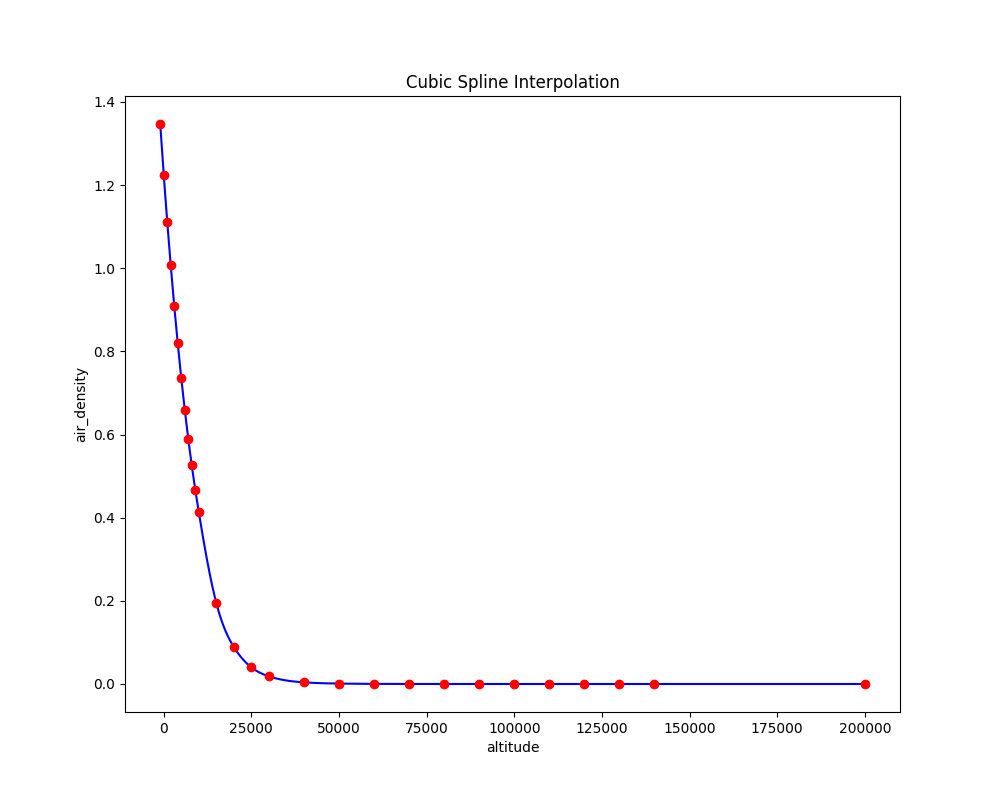
\includegraphics[width=1\textwidth]{images/cubic-spline.png}
\caption{Visualization of the Cubic Spline approximation function} \label{cubic_spline}
\end{figure}












%%%%%%%%%%%%%%%%%%      EARTH     %%%%%%%%%%%%%%%%%%%%%%

\subsection{Round Earth - Coordinate Reference System}

An essential aspect of the simulation is the coordinate reference system employed. In simpler simulations, a flat Earth model is typically used, where the y and x axes are perpendicular to each other, and movements and forces are defined accordingly. For instance, gravity acts vertically downward, perpendicular to the x-axis.

However, more detailed simulations require the assumption of a spherical Earth model. In our simulation, we incorporate this at two different levels.

\textbf{\\Partial Round Earth Model\\}
By default, we simulate using a standard flat Earth reference system. We track the Earth's angle (\(\theta\) in Fig. \ref{round_earth_vector}) to later adjust the horizontal distance traveled to fit the flat Earth model accurately. To this end, we might use the arc length formula:
\begin{equation}
    \theta = \frac{l}{r} \quad \Leftrightarrow \quad l = r \cdot \theta
\end{equation}
where \( l \) represents the arc distance and \( r \) denotes the radius of the circle. To find the traveled angle during the simulation, we increment the angle at each step using the formula:
\begin{equation}
    \theta_i = \frac{x_i - x_{i-1}}{R_{\text{Earth}} + y_i}
\end{equation}
And thus, having the angle and the altitude, we can calculate the distance using the previous arc length equation.

\textbf{\\Complete Round Earth Model\\}
Another simulation option in the app is to simulate a complete round Earth, including movement in the y-axis. To achieve this, we consider the base vectors of the ODE system that define our model. In this case, we have derivatives for positions and velocities, which are influenced by accelerations. By adjusting the direction of the acceleration vector to transition from a flat Earth to a round Earth model, we can accurately simulate a round Earth.

For example, as shown in Fig. \ref{round_earth_vector}, let's consider a position in the diagonal of the y-x orthogonal reference frame, where we are moving horizontally. In a flat Earth model, this horizontal vector is parallel to the x-axis. However, in a round Earth model, this vector is parallel to the tangent of the Earth's surface at that point. We can adapt this vector using trigonometry to find its y and x components.

Similarly, a vector pointing downwards in a flat Earth model, which is perpendicular to the x-axis, in a round Earth model represents a vector perpendicular to the tangent of the Earth's surface at that point. This downward vector thus points towards the center of the Earth, at the origin (0,0).


\begin{figure}
\centering
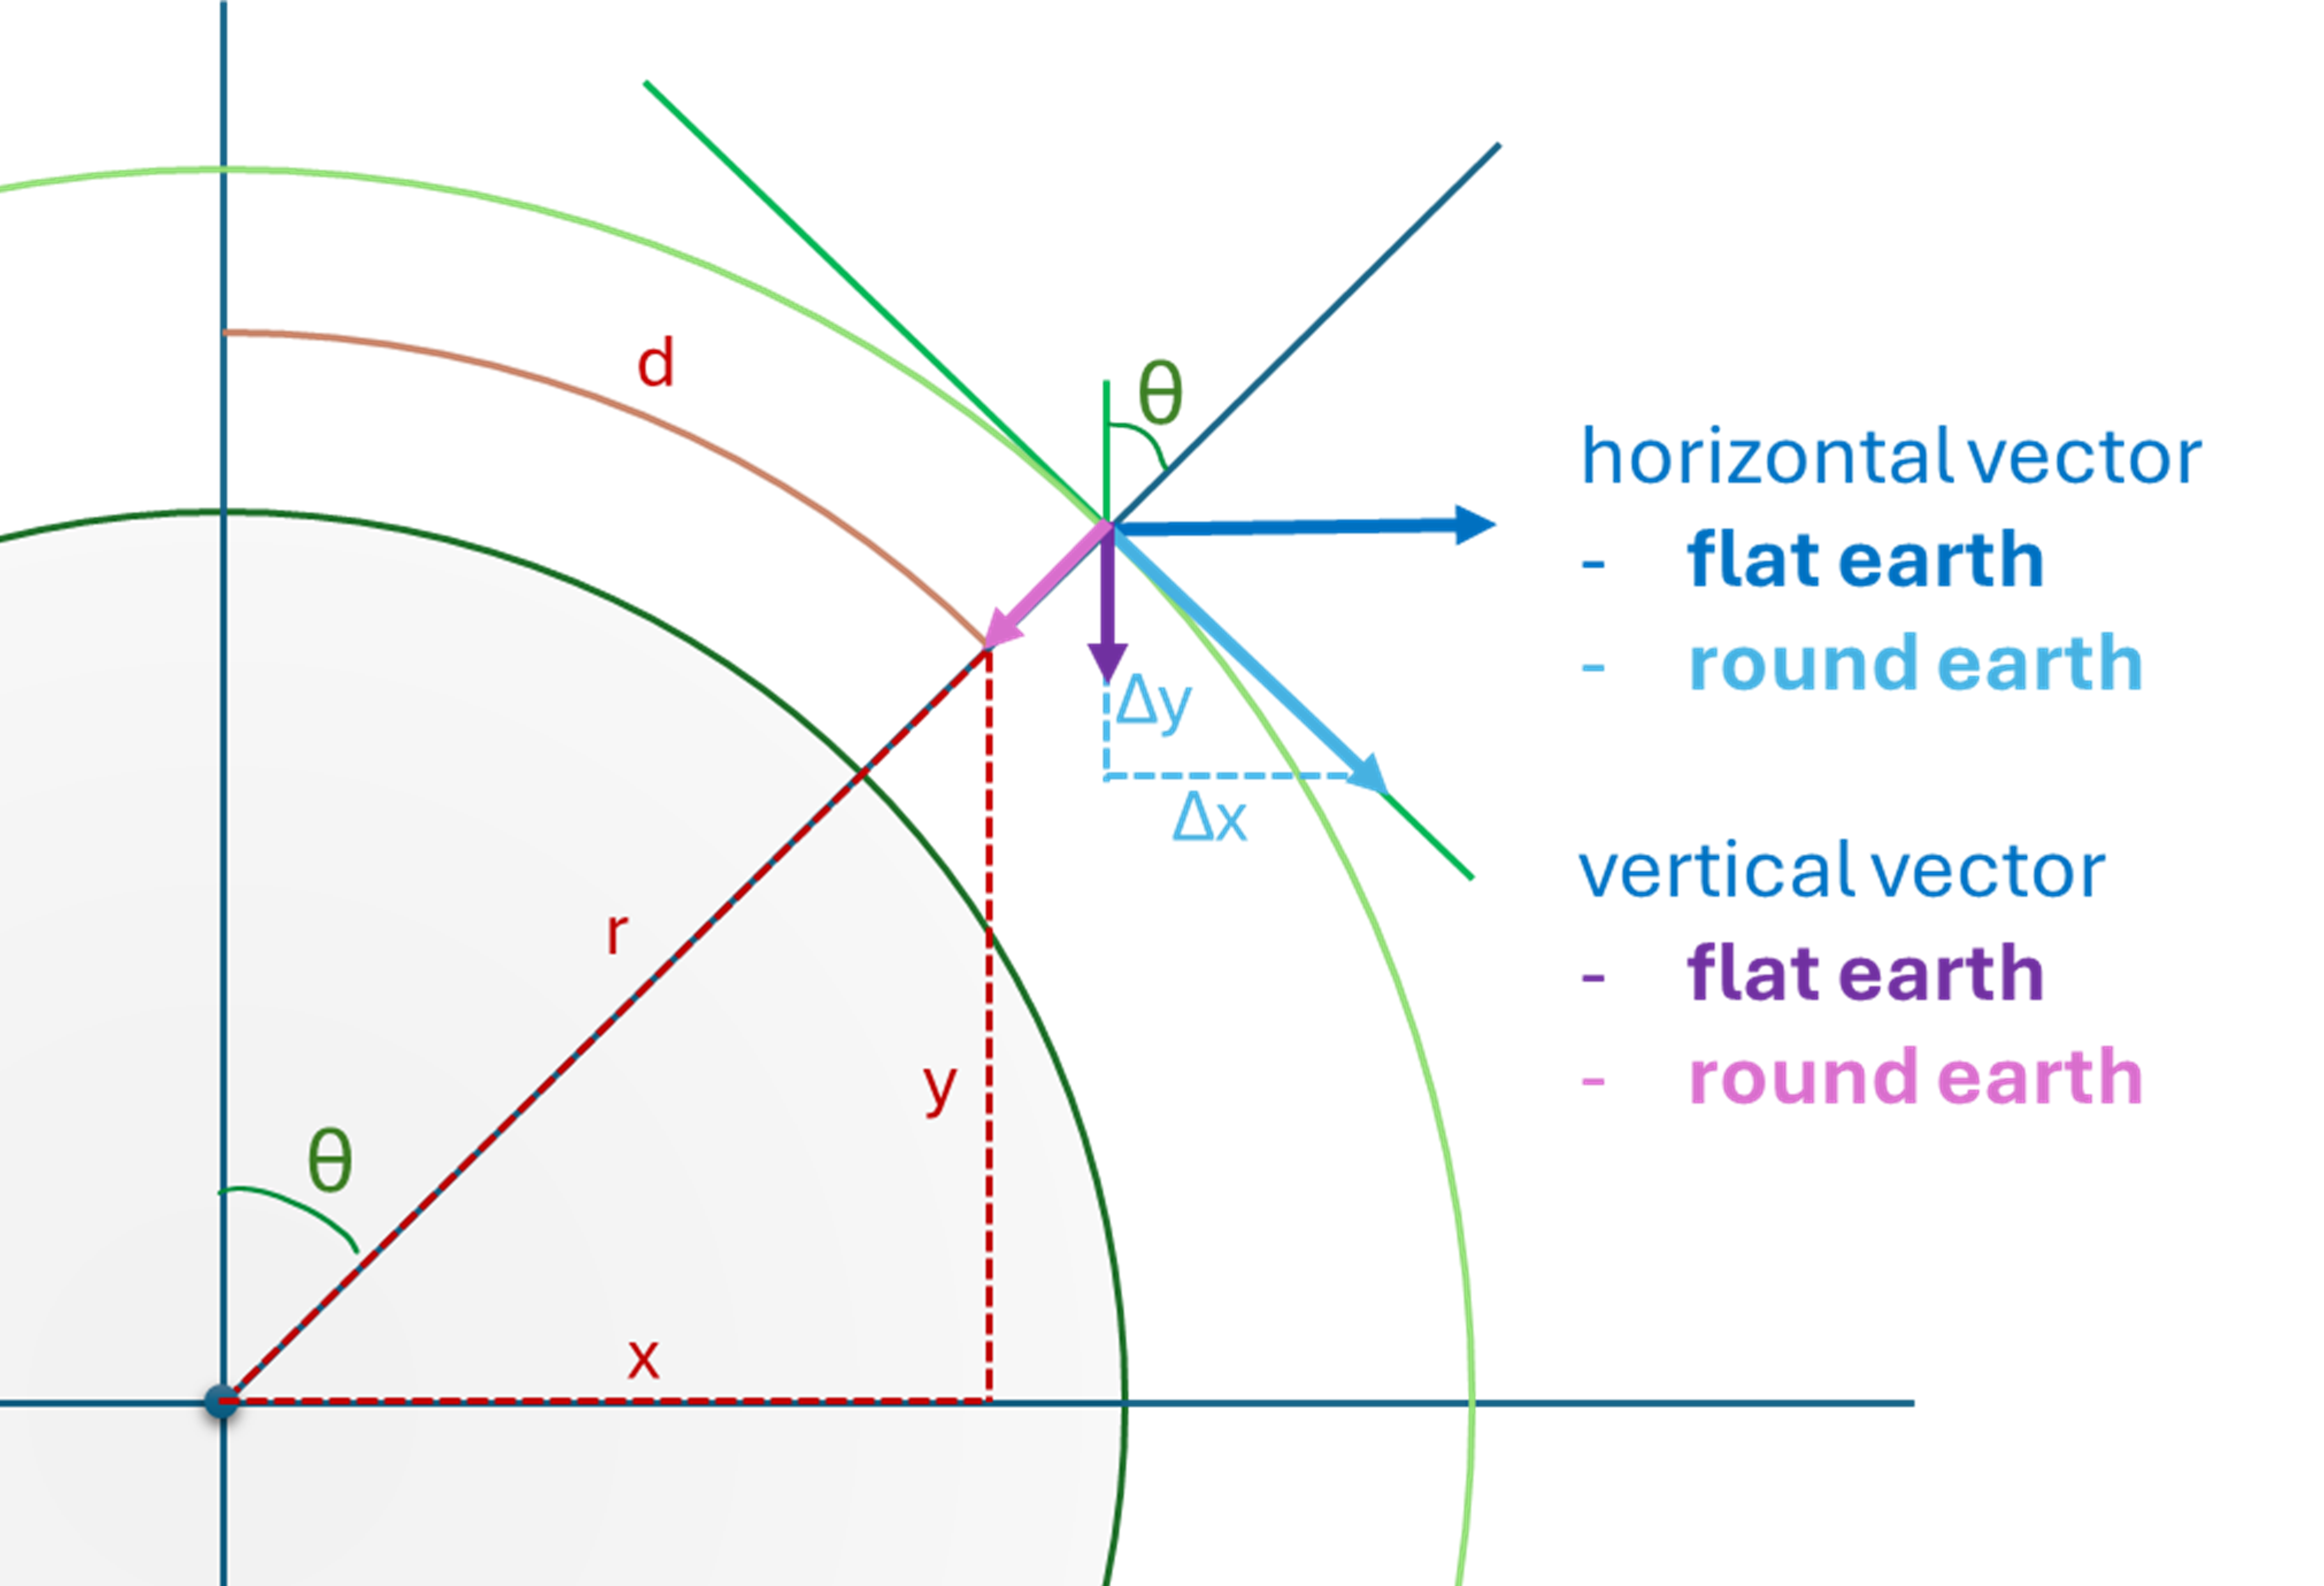
\includegraphics[width=0.75\textwidth]{images/round earth vector conversion.png}
\caption{Flat Earth - Round Earth vector and position conversions} \label{round_earth_vector}
\end{figure}

To convert a vector from a flat Earth model to a round Earth model, we use trigonometry to find the correct y and x components. The following code snippet demonstrates how to convert x and y steps from a flat Earth model to x and y steps in a round Earth model, given the Earth angle, \(\theta\):

\begin{minted}[frame=lines, bgcolor=verylightgray, fontsize=\small, linenos, numbersep=1pt]{python}
def make_round_earth (x_step, y_step, theta):
    x_round_step = y_step * np.sin(theta) + x_step * np.cos(theta)  
    y_round_step = y_step * np.cos(theta) - x_step * np.sin(theta)  
    return x_round_step, y_round_step
\end{minted}

This approach allows us to seamlessly run the simulation by simply modifying the base vector used in our system of ODE equations. This adjustment cascades through subsequent ODEs, enabling movement within a round-earth model.

Ultimately, we only need to visualize the x and y positions within the context of the round earth model. To convert the horizontal position to the flat earth model, we follow the method discussed earlier. When converting the y altitude from flat earth to round earth, as illustrated in Fig. \ref{round_earth_vector}, we simply calculate the distance from the position to the center of the earth, located at the origin of the reference point (0,0). For this, we use the Pythagorean theorem, where x and y values serve as the catheti, and the hypotenuse represents the distance.






%%%%%%%%%%%%%%%%%%      PARACHUTE     %%%%%%%%%%%%%%%%%%%%%%

\subsection{Parachute Deployment}

In addition to the ballistic simulation of capsule reentry, our model includes the deployment of a parachute under specific conditions: the altitude must be below 1,000 meters, and the velocity under 100 m/s. This parachute deployment significantly decelerates the capsule, which would otherwise land at approximately 85 m/s due to its own drag and lift components. With the parachute deployed, its additional drag force reduces the descent speed to around 25 m/s, resulting in a softer landing\footnote{This velocity of 25 m/s, or about 90 km/h, is still a very fast landing, so it is necessary to target a landing zone above water to reduce impact problems.}

\begin{figure}[h]
\centering
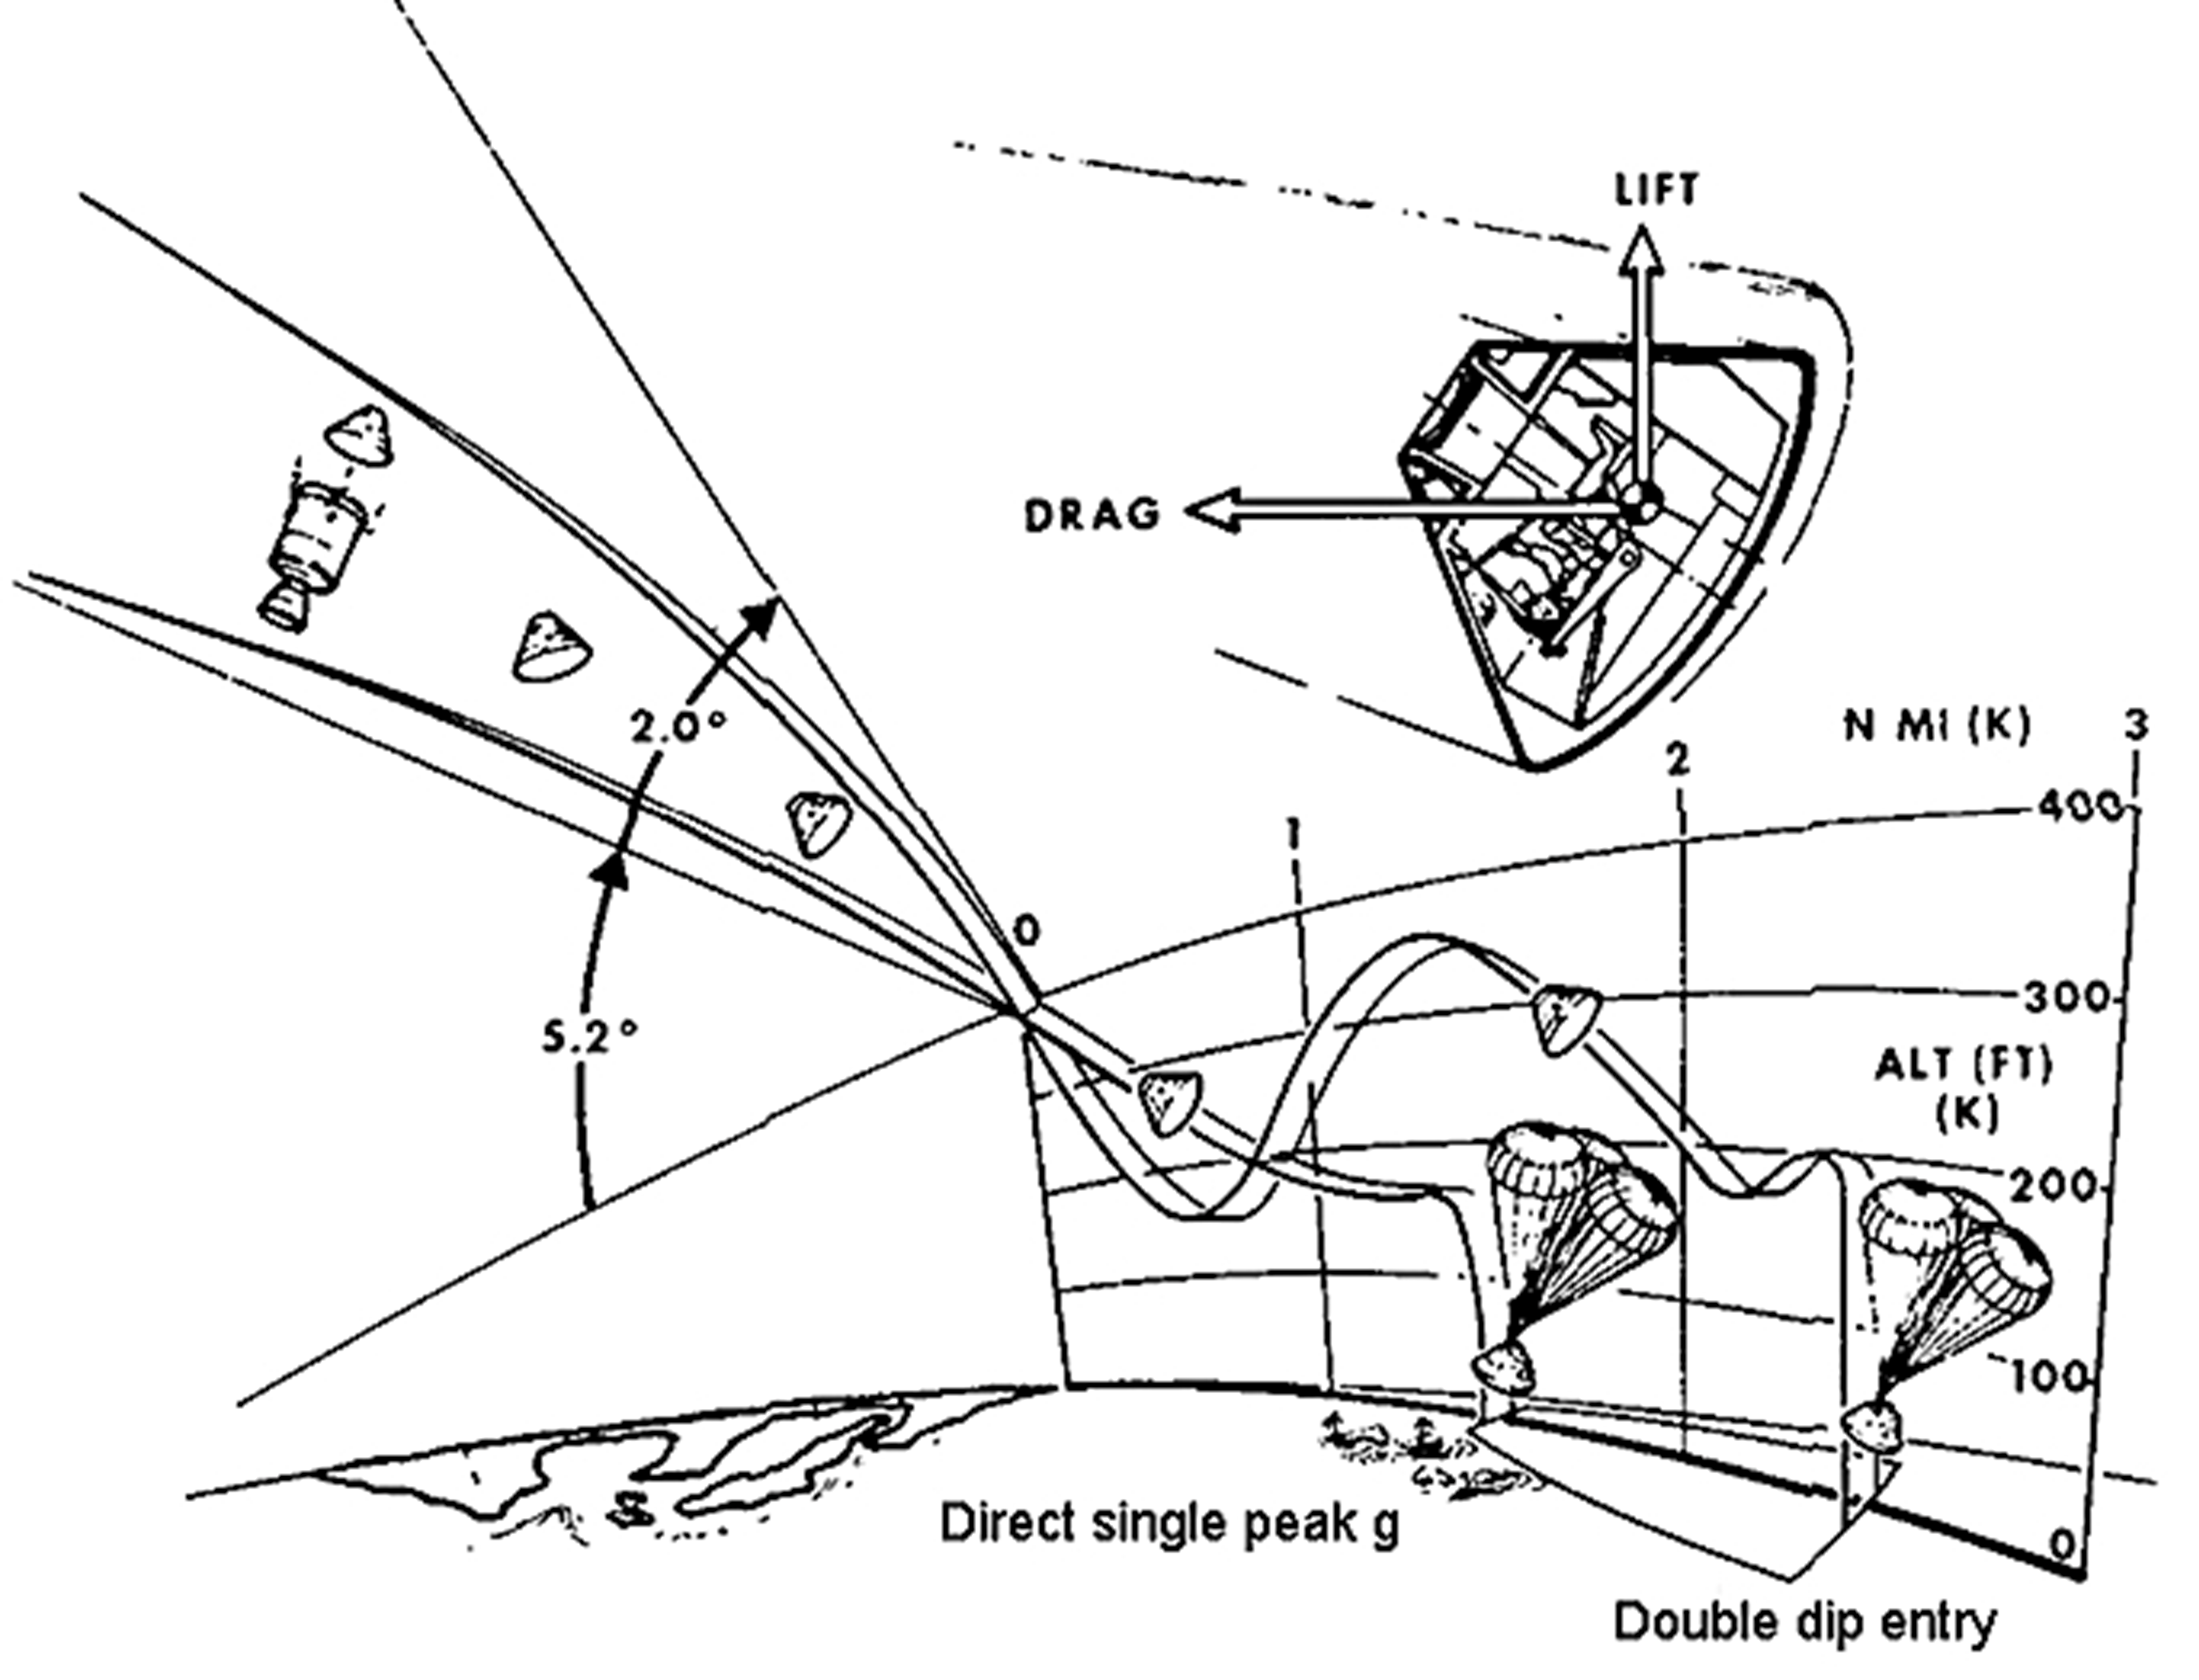
\includegraphics[width=0.6\textwidth]{images/parachute_draw.png}
\caption{Schematic of reentry trajectory with parachute deployment \cite{reentry_matters}}
\label{parachute_draw}
\end{figure}





%%%%%%%%%%%%%%%%%%      NOT CONSIDERED     %%%%%%%%%%%%%%%%%%%%%%

\subsection{Assumptions}

Several aspects were not considered in the simulation:

\textbf{\\Earth:\\}
In reality, the Earth is not perfectly circular but rather elliptical. However, for the model, we assume a perfect circular shape.

Additionally, the Earth's gravitational potential is not uniform due to its geoid shape, resulting in irregular gravitational forces across its surface. In the model, we assume uniform gravitational force along the surface, accounting only for changes with increasing altitude \cite{mazyku_optimum_reentry}.

During reentry simulations, Earth is assumed to be stationary and non-rotating. Therefore, factors like the Coriolis force, which deflects moving objects, and the centrifugal force due to Earth's spin are not considered. This simplification allows us to focus solely on gravitational effects and atmospheric dynamics without accounting for additional rotational influences on trajectory and atmospheric behavior.


\textbf{\\Air:\\}
Wind effects were not incorporated into the simulation. Given that the air is assumed to be still, there is no wind force impacting the dynamics, particularly notable after the parachute deployment. Consequently, neither drag nor lift calculations account for any wind influence.

\textbf{\\Aircraft:\\}
Although the angle of attack adjustment might be used to increase vertical lift automatically, the aircraft does not undergo any other maneuvers. The reentry simulation is entirely ballistic without any propulsion system. Additionally, the capsule remains stationary with respect to its reference frame, thus avoiding rotation and effects like the Magnus effect, which generates lateral forces perpendicular to the direction of movement \cite{returning_space}.






%%%%%%%%%%%%%%%%%%%%%%%%%%%%%%%%%%%%%%%%%%%%%%%%%
%%%%          METHODS OF SIMULATION          %%%%
%%%%%%%%%%%%%%%%%%%%%%%%%%%%%%%%%%%%%%%%%%%%%%%%%



\section{Methods of Simulation}
In this section, we will detail the mathematical methods employed for simulating the dynamics of the reentry capsule. Each method has specific characteristics that influence the accuracy and efficiency of the simulation.


\subsection{Forward Euler (Explicit)}

\textbf{ODEs / Slopes\\}
To simulate the evolution of a system, a reliable approach is to formulate a set of Ordinary Differential Equations (ODEs) that describe the predicted evolution or tendency of each variable. In our case, we focus on predicting the evolution of position and velocity, represented by variables \textbf{x}, \textbf{y}, \textbf{vx}, \textbf{vy}. These derivatives allow us to establish how these variables change over time. So by knowing the current state of these variables and their derivatives, we can simulate the trajectory of the capsule. Essentially, the derivatives indicate the slope or tendency of each variable at any given moment. With this information, knowing the current state and knowing the slope, we can predict where the capsule will be after a short interval of time \(\Delta\)t. The accuracy of our predictions improves with smaller time intervals \(\Delta\)t, ensuring a more precise simulation of the capsule's trajectory \cite{github_metaphysics}.

These systems of equations are often represented as vectors, denoted by symbols like \( \mathbf{S} \), \( \mathbf{U} \), or even a simple \( \mathbf{y} \) (which represents the entire system of equations rather than just a single variable \( y \), for instance, when using the solver\_ivp function in Python). This vector representation allows for a more flexible and concise implementation of the simulation dynamics. Here is an example of a system, where \( \mathbf{x} \), \( \mathbf{y} \), \( \mathbf{vx} \), and \( \mathbf{vy} \) represent the position and velocity variables, respectively \cite{github_channel}:

\begin{equation}
\mathbf{U}_{i+1} = \begin{bmatrix}
x_{i+1} \\
y_{i+1} \\
vx_{i+1} \\
vy_{i+1}
\end{bmatrix} =
\begin{bmatrix}
x_i + vx_i \cdot dt \\
y_i + vy_i \cdot dt \\
vx_i + ax_i \cdot dt \\
vy_i + ay_i \cdot dt
\end{bmatrix}
\end{equation}

This equation illustrates the update of state variables \( x \), \( y \), \( vx \), and \( vy \) from time step \( i \) to \( i+1 \) in discrete time increments \( dt \). Here, \( vx \) and \( vy \) represent the derivatives of \( x \) and \( y \), while \( ax \) and \( ay \) denote the derivatives of \( vx \) and \( vy \), indicating accelerations in the \( x \) and \( y \) directions, respectively. The formula for calculating these accelerations was discussed in the previous chapter.


\textbf{\\Forward Euler - Explicit\\}
The process described above is precisely what the Forward Euler method does: it computes the next state of variables based on the current state by calculating the slope and adding it multiplied by \( dt \) to the current state. It's also known as an explicit method because it computes the state variables directly from the previous state without iterative procedures or implicit calculations.

The Forward Euler method is renowned for its simplicity in implementation and understanding. In the following code snippet, we can observe how a forward Euler step is computed and how it is utilized to run a complete simulation:

\begin{minted}[frame=lines, bgcolor=verylightgray, fontsize=\small, linenos, numbersep=1pt]{python}
def forward_euler_step(Sk, p: Params, slope_f): 
    ''' Sk: values of the model in step k '''
    slopes = slope_f(Sk, p)
    Sk1 = Sk + slopes * p.dt
    return Sk1

def run_one_simulation(S0, p: Params, method_f):
    ''' S0: initial values of the model '''
    size = int(p.sim_max_time / p.dt + 1)
    S = np.zeros((size, S0.shape[0]), dtype=float)
    t = np.array([i * p.dt for i in range(size)])
    S[0] = S0
    for i in range(1, size):
        S[i] = method_f(S[i-1], p, reentry_slope)
        if (S[i][Y]) < RADIUS_EARTH:
            return S[:i+1], t[:i+1]
    return S, t
\end{minted}
\footnote{Having the function \texttt{run\_one\_simulation()} receive the concrete method function as an argument allows for more flexibility, as we can use the same code for running a simulation with forward Euler, backward Euler, etc.}


It also requires minimal computational resources. However, it is susceptible to instability, especially with larger time steps \( dt \), or when applied to stiff equations or systems with rapidly changing dynamics. For example, in simulations of oscillatory systems with damping, the solution should ideally tend towards zero. However, with larger time steps, the method can lead to numerical errors where the solution grows uncontrollably, deviating from physical expectations.


\subsection{Runge-Kutta (Explicit)}
To improve the prediction accuracy of movement over time, the Runge-Kutta method refines the approach used in the forward Euler method. While the forward Euler method calculates the slope only at time step \( i \) and uses it to predict the next step \( (i+1) \), the Runge-Kutta method calculates the slope at both time steps \( i \) and \( i+1 \), then averages them. This method is designed to provide a more accurate numerical approximation to the solution \cite{misc_rocket}.

The equations for \( k1 \) and \( k2 \) in the RK2 method are as follows:

\[
\begin{aligned}
k1 & = f(t_i, \mathbf{U}_i) \cdot dt, \\
k2 & = f(t_i + \frac{dt}{2}, \mathbf{U}_i + \frac{k1}{2}) \cdot dt,
\end{aligned}
\]

where \( f(t_i, \mathbf{U}_i) \) represents the slope vector at time \( t_i \) for state vector \( \mathbf{U}_i \).

These values \( k1 \) and \( k2 \) are then used to update the state vector \( \mathbf{U} \) from time step \( i \) to \( i+1 \) using the weighted average of slopes.

This method is more accurate than the explicit Euler method because it considers the variation of the function over the time interval \( dt \), providing a better numerical approximation to the solution. Expanding on this principle, Runge-Kutta methods offer different orders to enhance accuracy, making them highly effective for a wide range of simulation tasks \cite{github_reentry}.


\textbf{\\Python solver\_ivp\\}
For its versatility, Runge-Kutta is the default method used by Python's \texttt{solve\_ivp} (defaulting to Runge-Kutta 'RK45'). Other available options include 'RK23', 'DOP853', 'Radau', and 'BDF' for stiff problems. This solver runs the simulation automatically, making it both easy to use and precise. We only need to pass the slope function that calculates the derivatives of each variable of the model (all first-order ODEs), set an initial condition, specify an array with all the times to test, and run it. Here is an example of code implementation with an early stop condition \cite{misc_rocket}:

 
\begin{minted}[frame=lines, bgcolor=verylightgray, fontsize=\small, linenos, numbersep=1pt]{python}
from scipy.integrate import solve_ivp

params = None
acceleration_f = None

def solve_ivp_sim(t, Y0):
    x, y, vx, vy, = Y0
    v = np.sqrt(vx**2 + vy**2)
    ax, ay = acceleration_f(Y0, params)
    return [vx, vy, ax, ay]

def event_conditions(t, Yk):
    return Yk[Y] - RADIUS_EARTH

def solver_ivp (Sk, Mk, p: Params, get_acceleration_f):
    global params, acceleration_f
    params = p
    acceleration_f = get_acceleration_f
    
    size = int(p.sim_max_time / p.dt + 1)
    t = np.array([i * p.dt for i in range(size)])

    # Stop the integration when this event occurs
    event_conditions.terminal = True  
    # Look for a decreasing y position
    event_conditions.direction = -1   

    sol = solve_ivp(
                solve_ivp_sim,                      # slopes function
                [0, size],                          # time span
                y0=[Sk[X], Sk[Y], Sk[VX], Sk[VY]],  # initial state  
                t_eval=t,                           # times to run
                events=event_conditions,            # stop condition
                dense_output=True)  
    t = sol.t
    S = sol.y.T
    return S, t
\end{minted}




\subsection{Implicit Euler}
As stated, Runge-Kutta RK45 is a versatile method and thus is the default method for \texttt{solve\_ivp}. However, for stiff problems, rapid-changing dynamics, or situations where we need to use larger time steps, it's better to use implicit methods like Radau or BDF.

Unlike the forward Euler method, where we use the slope at the current state to predict the next state, or Runge-Kutta methods, which use the slope at both states and average them, implicit methods use the slope at \(i+1\) to predict the value of that same state \(i+1\), as described in the following formula \cite{hornik_optimization}:
\begin{equation}
    U_{k+1} = U_k + f(U_{k+1}, t_{k+1}) \cdot dt
\end{equation}

This results in the variable we are trying to solve for appearing on both sides of the equation, which is why it is termed an "implicit method." To solve this equation, we can rearrange all terms to one side, setting the equation to zero and finding its roots. To that end, in this simulation, we apply the Newton-Raphson method.

\textbf{\\Newton Method\\}
The Newton-Raphson method aims to find the root of the non-linear equation \( R(v) = 0 \), where \( R(v) \) is the residual given by the difference between the left-hand side and the right-hand side of the following equation. In each iteration, we calculate the correction \( \Delta v \) and adjust \( v \) to approximate the solution, as stated in the following formula \cite{hornik_optimization}.

\begin{equation}
\frac{I}{\Delta t} - J(f(v,t^{(k+1)})) \Delta v = -\left(\frac{v - u^k}{\Delta t} - f(v, t^{(k+1)})\right)
\end{equation}

\textbf{Jacobian Term:}
This term combines the identity matrix scaled by the inverse of the time step with the Jacobian matrix of the function of the system derivatives.
\begin{itemize}
    \item \( I \): Identity matrix, used to preserve the scale of the term \( v/\Delta t \) in the calculation.
    \item \( \Delta t \): Time step interval used in the temporal integration.
    \item \( J(f(v, t^{k+1})) \): Jacobian matrix - the matrix of partial derivatives of the function \( f \) with respect to \( v \) at time \( t^{k+1} \), used to linearize the system of non-linear equations.
    \item \( \Delta v \): Correction vector of the state vector \( v \); it is the amount by which the vector \( v \) will be adjusted in the current iteration.
\end{itemize}

\textbf{Right-Hand Side Term - Residual(v):}
This term represents the difference between the current estimated solution and the previous solution adjusted by the time step, subtracted by the function \( f \).
\begin{itemize}
    \item \( v \): State vector at time \( t^{k+1} \); it is the solution we are trying to find for the next time step.
    \item \( u^k \): State vector at time \( t^k \) (previous step).
    \item \( \frac{v - u^k}{\Delta t} \): Represents the difference between the current approximated state \( v \) and the previous state \( u \), scaled by the time step. This is an approximation of the derivative of \( v \) with respect to time (\( \frac{dv}{dt} \)).
    \item \( f(v, t^{k+1}) \): Function of the derivatives or slopes of the system at time \( t^{k+1} \), calculated for the state \( v \) that we are approximating.
\end{itemize}

\textbf{\\Implementation:} To better understand the workings of the Newton method, let's consider a simple example with the following system of equations:
\[
\begin{aligned}
f_1(x,y) &= x^2 + y^2 - 4, \\
f_2(x,y) &= e^x + y - 1.
\end{aligned}
\]
We aim to find the vector \( \mathbf{v} = (x, y) \) such that both \( f_1(\mathbf{v}) \) and \( f_2(\mathbf{v}) \) equal zero. To achieve this, we define the function \( \mathbf{f} \) and its derivative. When dealing with a system of equations, we use the Jacobian matrix to represent the partial derivatives with respect to all variables (in this case, \( x \) and \( y \)) of all system functions (in this case, \( f_1 \) and \( f_2 \)). Starting with an initial estimate of the root \( \mathbf{v} \), we iteratively update this estimate based on the ratio of the function value to its derivative at the current step estimate:
\[
\mathbf{x}_{n+1} = \mathbf{x}_n - \frac{f(\mathbf{x}_n)}{f'(\mathbf{x}_n)}
\]
In our case, having a system of equations and using the Jacobian matrix:
\[
\mathbf{x}_{n+1} = \mathbf{x}_n - \frac{\mathbf{F}(\mathbf{X}_n)}{\mathbf{J}(\mathbf{X}_n)}
\]

\noindent The following code snippet illustrates this implementation:

\begin{minted}[frame=lines, bgcolor=verylightgray, fontsize=\small, linenos, numbersep=1pt]{python}
def f(v): 
    ''' returns the image of vector v = (x,y) '''
    x, y = v
    return np.array([x**2 + y**2 - 4, np.exp(x) + y - 1])

def jacobian_f(v): 
    ''' returns matrix with partial derivatives of the system ''' 
    x, y = v
    return np.array([[2*x, 2*y], [np.exp(x), 1]])


def newton_method_system(v0, max_iter=1000, epsilon=1e-6, dt=0.1):
    ''' iteratively find an estimation to the roo '''
    v = np.array(v0) # initial estimative (we use the previous step) 
    Idt = np.eye(len(v))/dt # Identity matrix to apply the given step dt
                            # to the Jacobian matrix 
    for i in range(max_iter):
        R_v = f(v) # calculate image of the estimative (the residual)  
        if np.linalg.norm(R_v) < epsilon: # if good approximation, break
            break       # for more precise evaluation we can use 		
                        # if np.all(np.abs(Sk1) < epsilon): break
        J_f_v = jacobian_f(v) # calculate Jacobian matrix (derivatives)
        system_matrix = Idt - J_f_v # left term (adjusted to step size) 
        dv = np.linalg.solve(system_matrix, -R_v) 
            # having the system J(f(v))∆v = -R(v), 
            # we solve for ∆v = -R(v)/J(f(v))            
        v += dv    # adding ∆v we have: X(n+1) = x(n) - f(x)/f'(x)   
    return v

v0 = [0.5, 0.5] # Initial estimative
root = newton_method_system(v0)
print(f"Root found: v = {root}")
\end{minted} 

Now, in complex systems, we might not have a precise equation to represent the model. For example, with constant gravity, we could use the kinematic equation for position x as a function of time, and directly obtain \( x \):

\begin{equation}
x = x_0 + v_0 t + \frac{1}{2} a t^2
\end{equation}

However, when gravity varies with altitude, and drag and lift forces change with air density (which also varies with altitude), we don't have a direct equation to represent the system. Instead, we use an approximation involving derivatives, as represented by the right side of the initial equation \cite{newton_raphson_method}:

\begin{equation}
R(v) = \left( \frac{v - u^k}{\Delta t} - f(v, t^{k+1}) \right)
\end{equation}

\noindent which we can implement directly in code, using the same slope function that describes the system, as we did for the explicit Euler method:

\begin{minted}[frame=lines, bgcolor=verylightgray, fontsize=\small, linenos, numbersep=1pt]{python}
def get_residual_vector(Sk, Sk1, p: Params, slope_f):
    slopes = slope_f(Sk1, p) 
    res_vector = (Sk1 - Sk)/p.dt - slopes
    return res_vector
\end{minted}


\textbf{\\Jacobian Matrix\\}
Finally, the missing piece is to actually build the Jacobian matrix. To do this, we calculate the partial derivatives of each function with respect to each variable. In the case of our simulation: 

\[
J = \begin{bmatrix}
        \frac{\partial f_1}{\partial x} & \frac{\partial f_1}{\partial y} & \frac{\partial f_1}{\partial vx} & \frac{\partial f_1}{\partial vy} \\
        \frac{\partial f_2}{\partial x} & \frac{\partial f_2}{\partial y} & \frac{\partial f_2}{\partial vx} & \frac{\partial f_2}{\partial vy} \\
        \frac{\partial f_3}{\partial x} & \frac{\partial f_3}{\partial y} & \frac{\partial f_3}{\partial vx} & \frac{\partial f_3}{\partial vy} \\
        \frac{\partial f_4}{\partial x} & \frac{\partial f_4}{\partial y} & \frac{\partial f_4}{\partial vx} & \frac{\partial f_4}{\partial vy}
    \end{bmatrix}
\]

Here, each row corresponds to a function \( f_i \) and each column corresponds to a variable \( x, y, vx, vy \). To find the partial derivatives, one can use various tools such as Wolfram Alpha, MATLAB, or Python libraries like SymPy. These tools can automate the process of differentiation, especially when dealing with complex functions or systems of equations. With the partial derivatives in hand, we proceed to implement the Jacobian matrix in our code, as demonstrated in the following snippet:

\begin{minted}[frame=lines, bgcolor=verylightgray, fontsize=\small, linenos, numbersep=1pt]{python}
def get_jacobian_matrix(Sk, p: Params):
    '''Returns the Jacobian matrix.'''
    x, y, vx, vy = Sk
    v = np.sqrt(vx**2 + vy**2)
    v = 1e-20 if v == 0 else v

    # Air density
    rho = air_dens_f(y - RADIUS_EARTH)
    d_rho = air_dens_f.derivative()(y - RADIUS_EARTH)

    # Constants for drag of capsule and parachute, and lift of capsule 
    Dc = -0.5*p.capsule_A*p.capsule_Dc/p.c_mass
    Dp = -0.5*p.parachute_A*p.parachute_Dc/p.c_mass
    Lc = 0.5*p.capsule_A*p.capsule_Lc/p.c_mass
    
    # Build the Jacobian matrix
    J = np.zeros((4, 4))

    # vx partial derivatives 
    J[0][2] = 1
    
    # vy partial derivatives
    J[1][3] = 1

    # ax partial derivatives
    J[2][1] = (Dc*d_rho*vx*v) + (Dp*d_rho*vx*v)
    J[2][2] = ((Dc*rho*(2*vx**2+vy**2))/v) + ((Dp*rho*(2*vx**2+vy**2))/v)
    J[2][3] = ((Dc*rho*vx*vy)/v) + ((Dp*rho*vx*vy)/v)

    # ay partial derivatives
    J[3][1] = (Dc*d_rho*vy*v) + (Dp*d_rho*vy*v) \
                + (Lc*d_rho*(vx**2 + vy**2)) + (2*G_M*p.c_mass)/(y)**3
    J[3][2] = (Dc*rho*vx*vy/v) + (Dp*rho*vx*vy/v) + (2*Lc*rho*vx)
    J[3][3] = (Dc*rho*(2*vy**2 + vx**2)/v) + (Dp*rho*(2*vy**2 + vx**2)/v) \
                + (2*Lc*rho*vy)

    return J
\end{minted}


\textbf{\\Implicit method results:\\}
Although harder to implement and understand, and computationally heavier, implicit methods offer distinct advantages, particularly in simulating stiff systems. Explicit methods are more prone to producing unstable results when simulating stiff equations, especially when varying the size of time steps (dt). Stiff equations involve components that evolve at significantly different rates, necessitating extremely small time steps for explicit methods to maintain stability. E.g., in damped oscillatory systems where oscillations tend toward zero, using explicit methods with larger time intervals can lead to oscillations growing over time. In contrast, implicit methods can maintain stability and accuracy in such scenarios.

The increased stability of implicit methods enables the use of larger time steps when necessary to expedite simulations without compromising stability. This capability proves particularly advantageous in simulations prioritizing computational efficiency, where using smaller time steps with explicit methods would be impractical.






%%%%%%%%%%%%%%%%%%%%%%%%%%%%%%%%%%%%%%%%%%%%%%%%%
%%%%          SIMULATION RESULTS             %%%%
%%%%%%%%%%%%%%%%%%%%%%%%%%%%%%%%%%%%%%%%%%%%%%%%%


\section{Simulation Results}

Having presented the physics and the mathematical methods to simulate the reentry of a capsule into Earth's atmosphere, we will now discuss observed results. This section encapsulates important details including code implementation, validation, and physical aspects.


\subsection{Round vs Flat Earth}
An important observation arises from our choice of reference system. When using a flat Earth model (where we only adjust horizontal distances to approximate a round Earth), all trajectories eventually land. This is because the Earth's surface is represented by the x-axis, which extends indefinitely. In this model, the simulation concludes with all trajectories reaching the surface, reflecting the infinite nature of the x-axis in this conceptualization. However, this model does not accurately reflect reality due to Earth's spherical shape. For instance, if we were to initiate a reentry trajectory with a launch angle of 0 degrees and an initial orbital velocity defined by the formula:

\[ v_{orbital} = \sqrt{\frac{G \cdot M_{earth}}{R_{earth}}} \]

we would theoretically enter orbit around Earth, maintaining a constant altitude indefinitely. This is because the orbital velocity \( v_{orbital} \) ensures that the centrifugal force, which counteracts gravity, balances perfectly with Earth's gravitational pull. As a result, the object would continuously fall towards Earth's surface due to gravity but also move tangentially with sufficient velocity to maintain a stable orbit, rather than descending directly to the ground as predicted by a flat Earth model.

This scenario highlights the discrepancy between the simplified flat Earth model and the actual orbital mechanics governed by gravitational forces around a spherical Earth. In Fig. \ref{orbit_round_earth}, we observe that the altitude remains nearly constant, with the simulation showing a slight decrease of approximately 2,000 meters over a traveled distance of 1,750,000 meters along the Earth's surface. Similarly, the velocity exhibits a minor increase of 5 m/s. The acceleration approaches zero in this scenario because the gravitational force balances the centrifugal force, leading to a stable orbital condition.


\begin{figure}
\centering
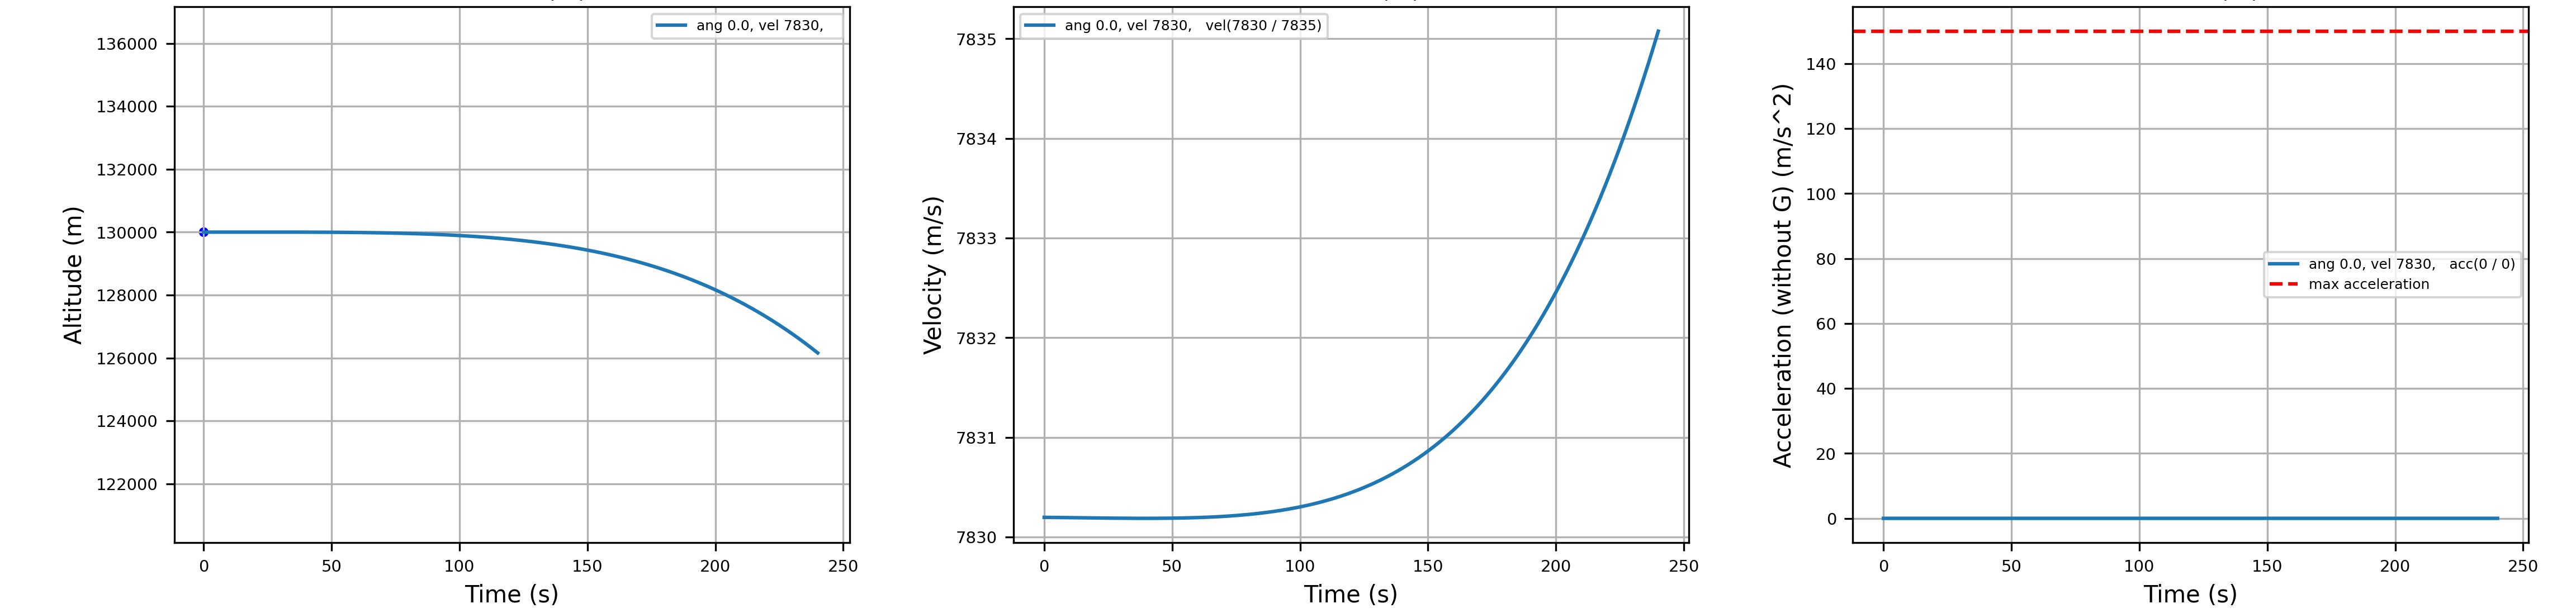
\includegraphics[width=1\textwidth]{images/orbit_round_earth.png}
\caption{Orbital velocity in \textbf{Round Earth} model} \label{orbit_round_earth}
\end{figure}

In contrast, in the flat Earth model, the trajectory is tangential to the Earth's surface, meaning that the y-coordinate remains unchanged. Consequently, the trajectory experiences a continual decrease in altitude, leading to descent into Earth's atmosphere. This descent highlights the effects of drag and lift, influenced by varying air density, as depicted in Fig. \ref{orbit_flat_earth}.

\begin{figure}
\centering
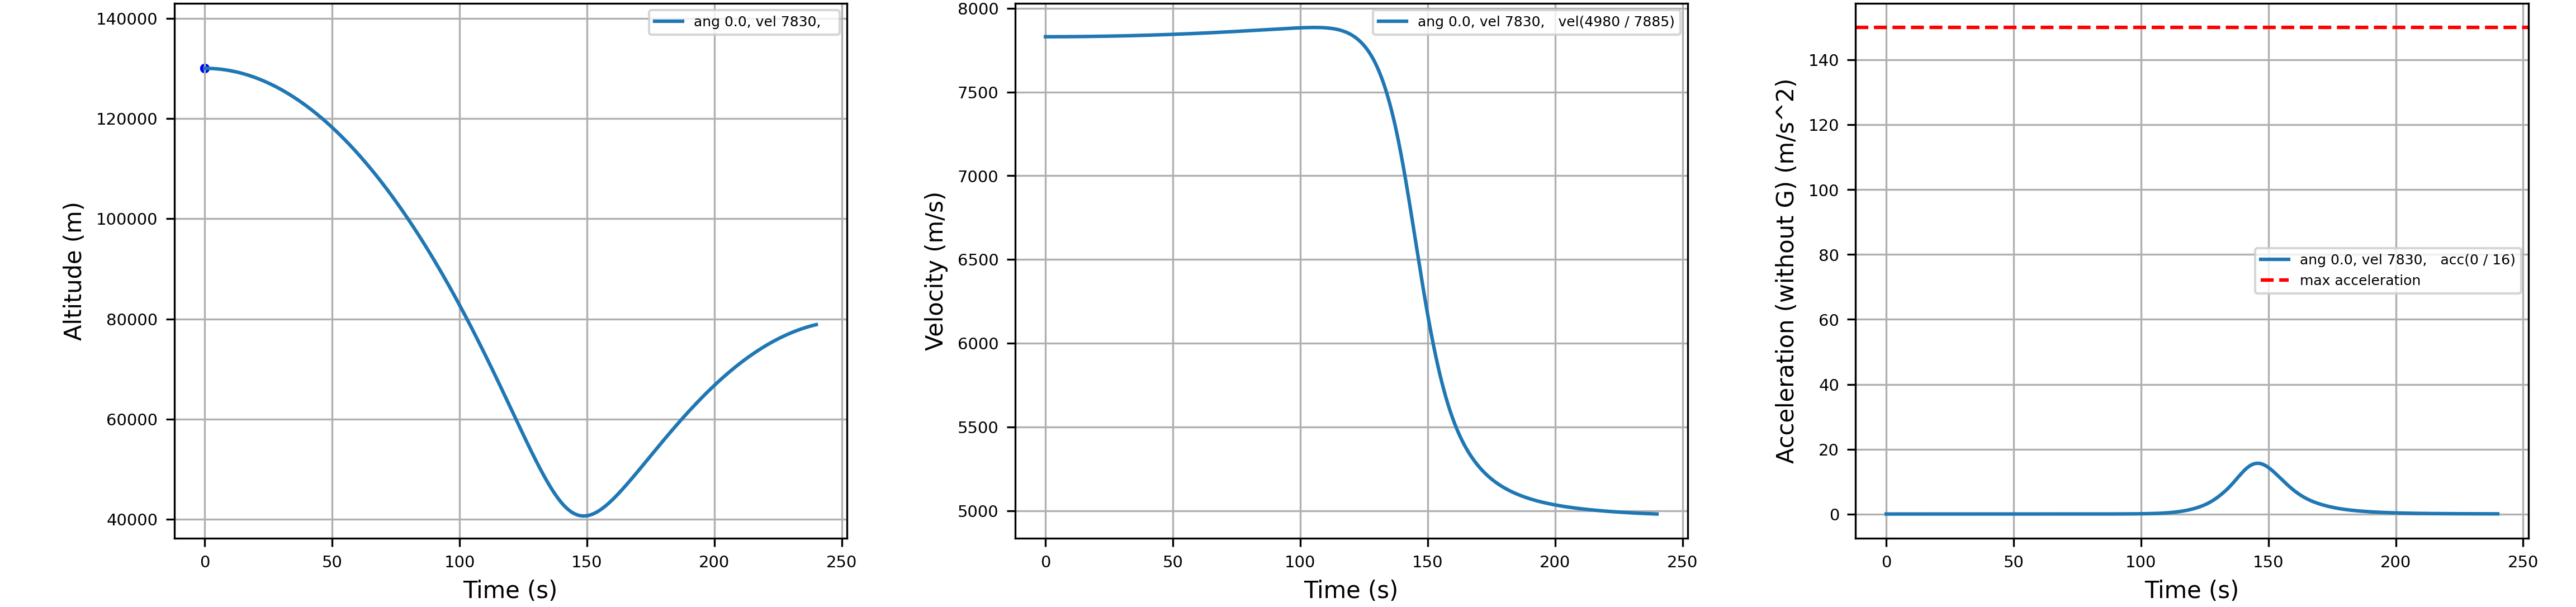
\includegraphics[width=1\textwidth]{images/orbit_flat_earth.png}
\caption{Orbital velocity in \textbf{Flat Earth} model} \label{orbit_flat_earth}
\end{figure}


\textbf{\\Effects of Drag and Lift:\\}

Another important consideration between the flat Earth and round Earth models is the effect of drag and lift forces. When a capsule reenters the atmosphere at high velocities, these aerodynamic forces increase proportionally to the square of the velocity \( v^2 \). Consequently, at greater velocities, the capsule may experience a significant rebound in the denser part of the Earth's atmosphere (typically starting around 60,000 meters, depending on the velocity and entry angle). 
And this phenomenon is observed in the flat Earth model but not as significantly as in the round Earth model. As illustrated in Fig. \ref{bounce_round_earth}, in the round Earth model, velocities of 12,000 m/s exhibit a bounce-back effect in the atmosphere and do not return. This can be observed in both the position plot on the left and the velocity plot in the center.

\begin{figure}
\centering
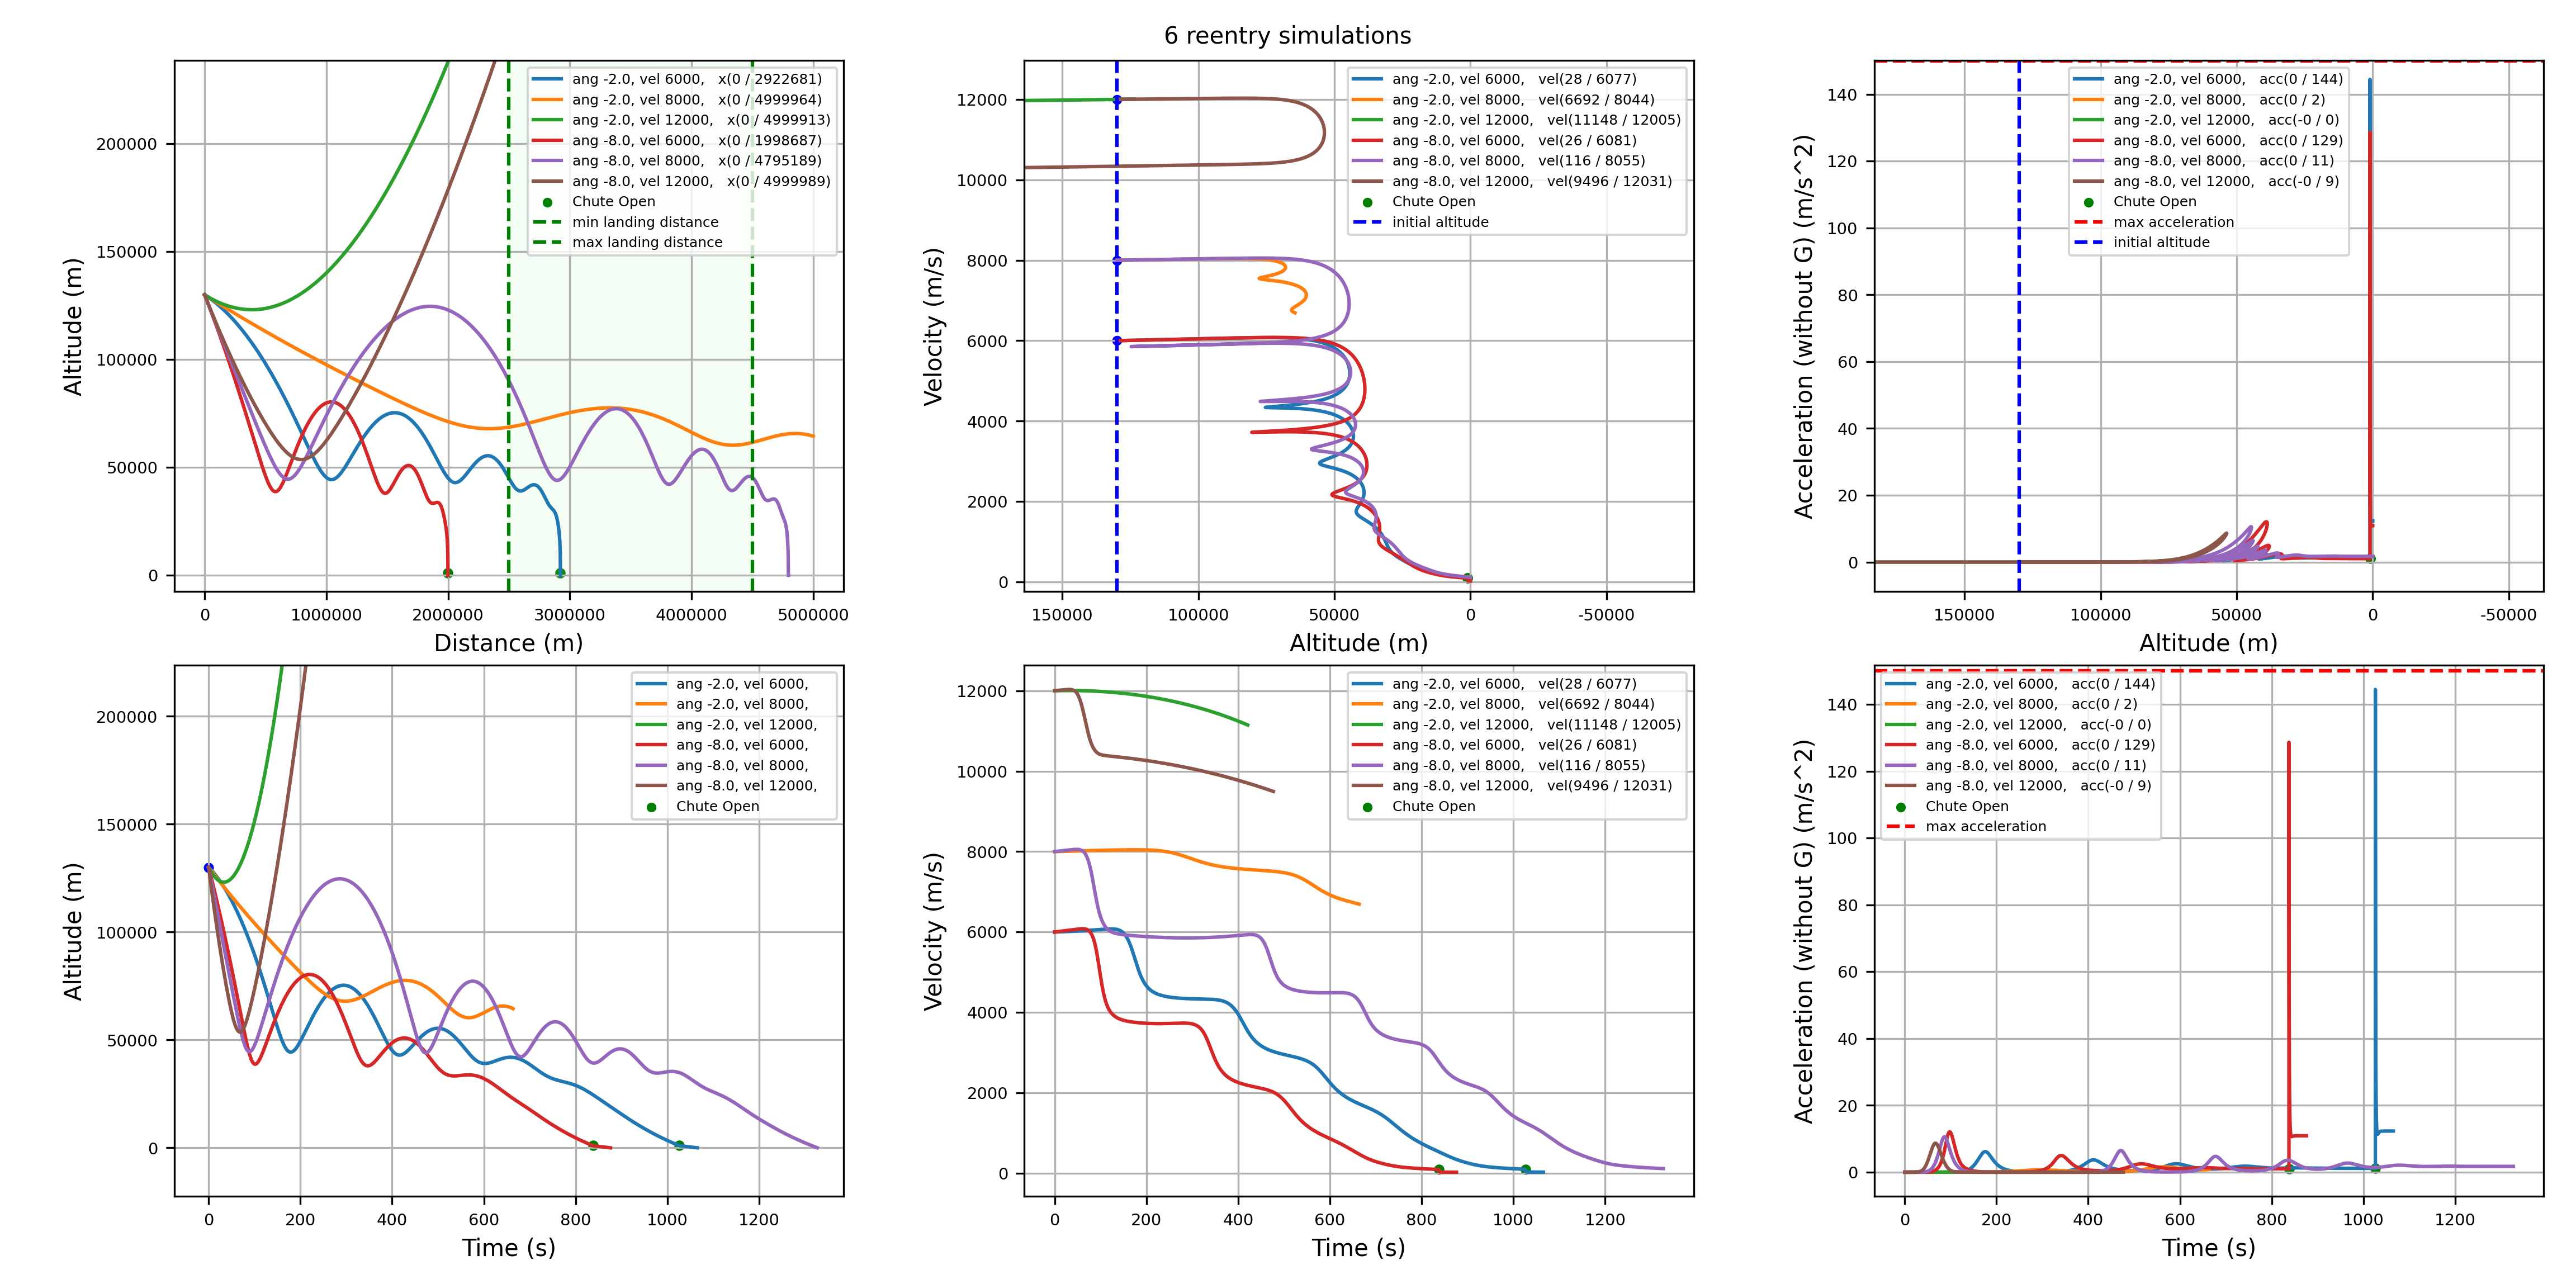
\includegraphics[width=1\textwidth]{images/bounce_round_earth.png}
\caption{Drag and Lift bouncing effect on \textbf{Round Earth} model} \label{bounce_round_earth}
\end{figure}

This phenomenon is not observed in the flat Earth model, as depicted in Fig. \ref{bounce_flat_earth}, where all trajectories return to Earth swiftly enough, often landing well before reaching the maximum landing distance boundary.


\begin{figure}
\centering
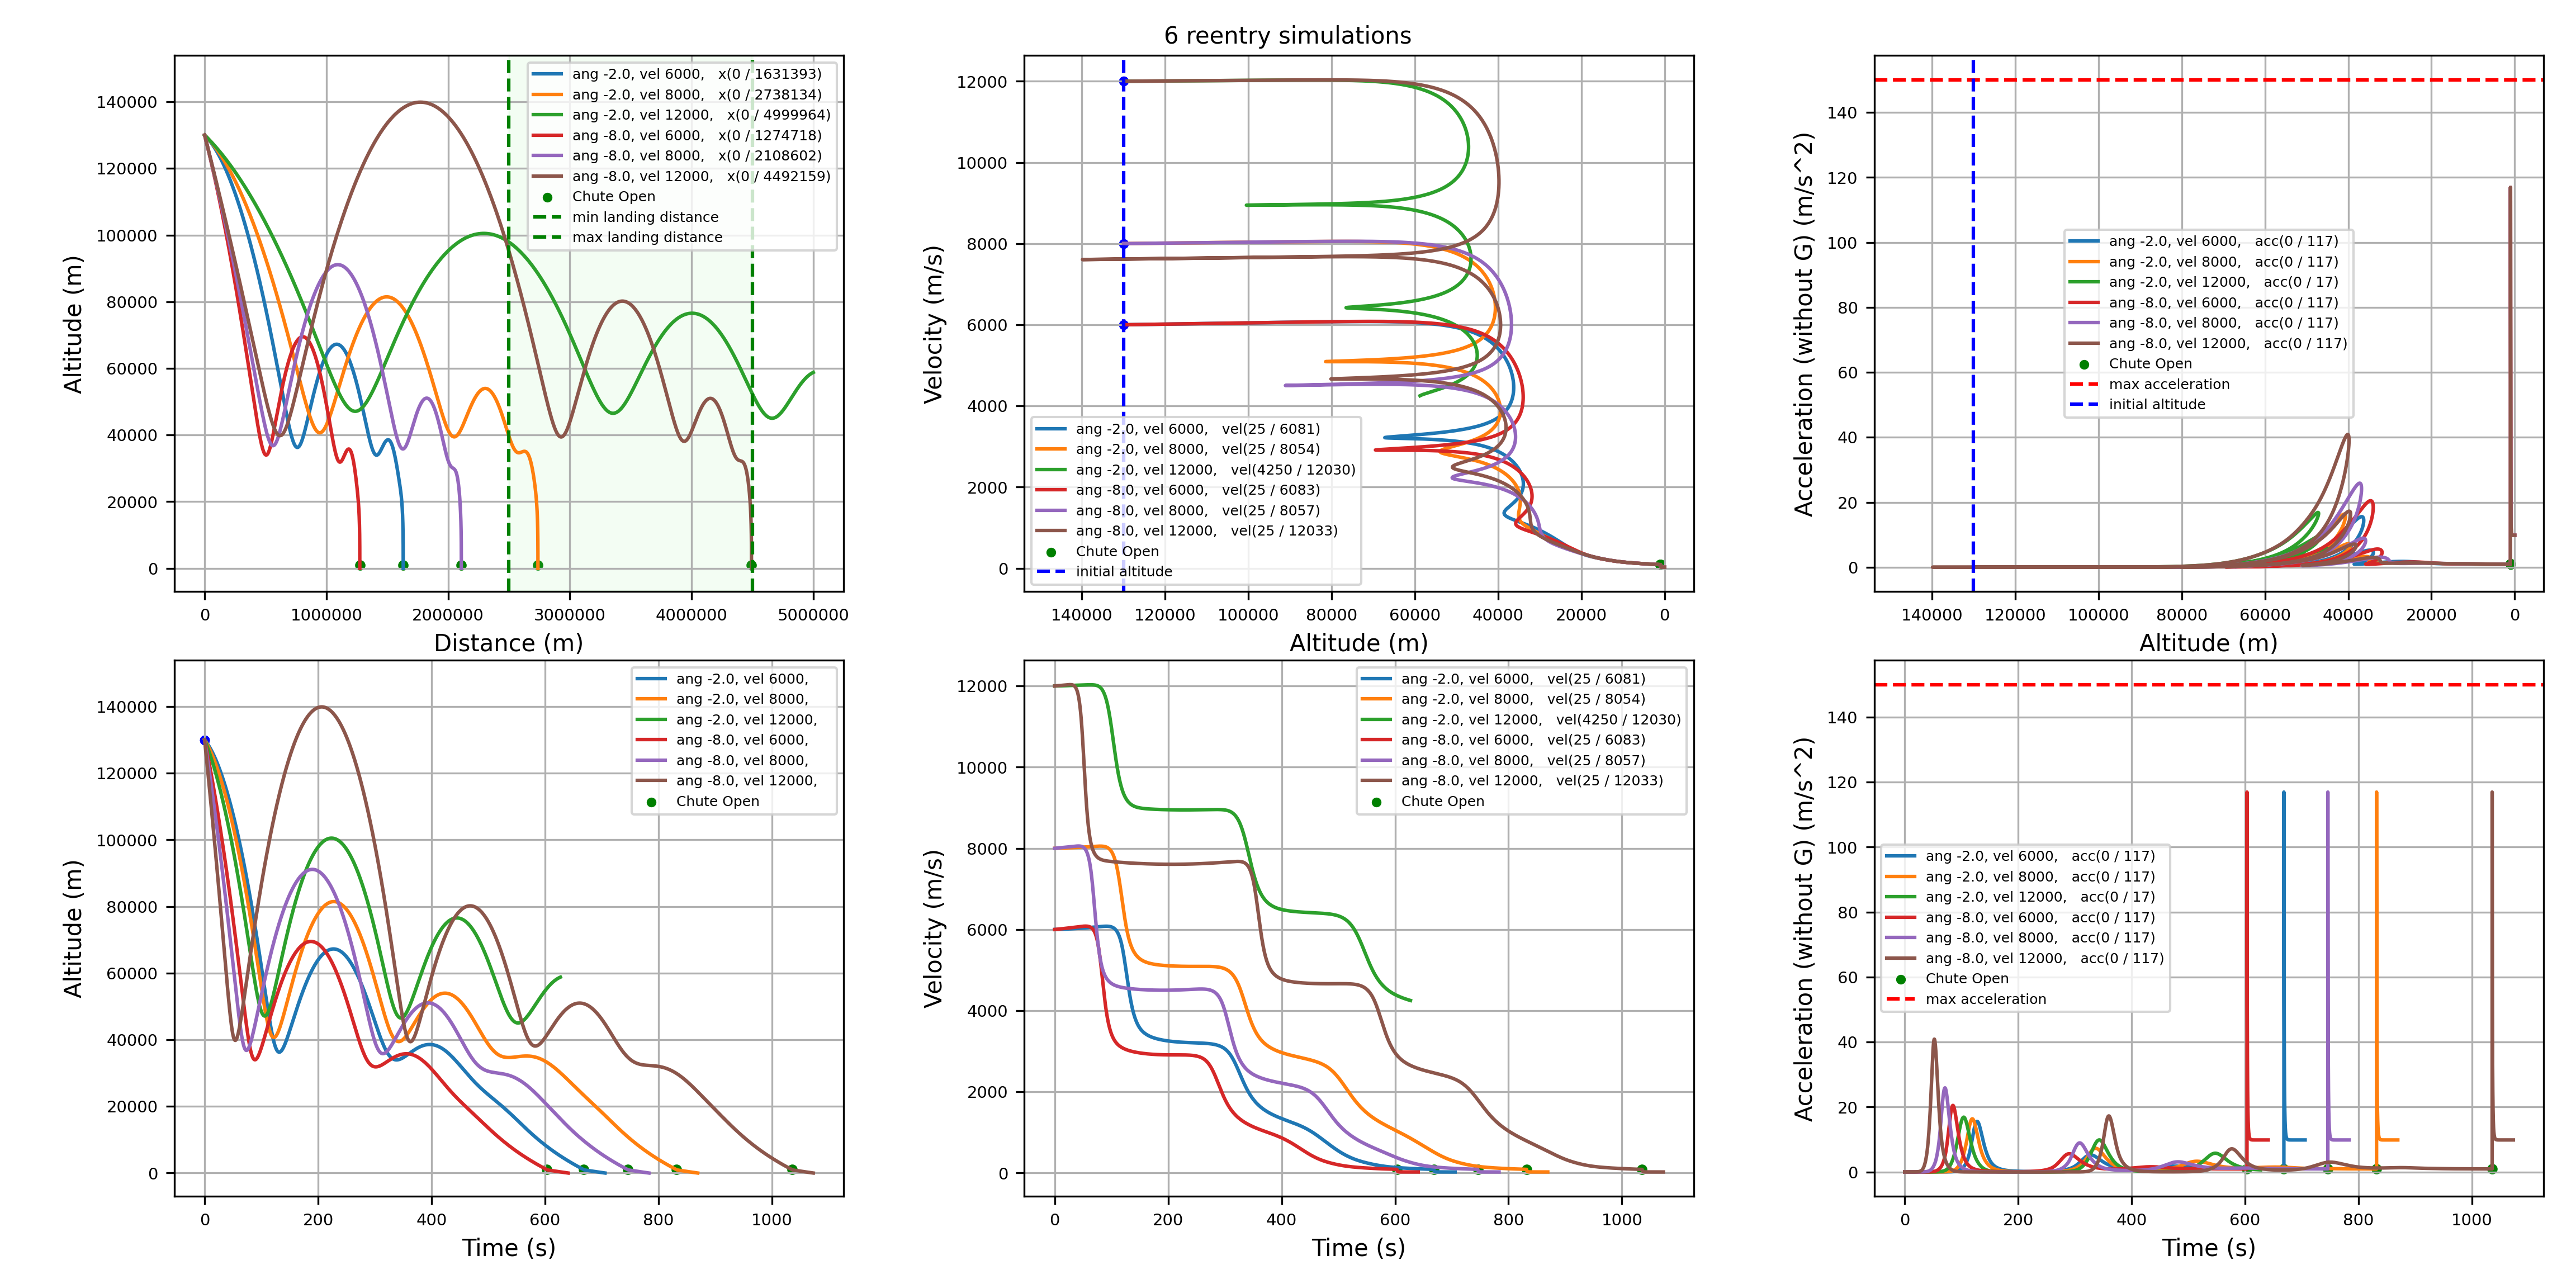
\includegraphics[width=1\textwidth]{images/bounce_flat_earth.png}
\caption{Drag and Lift bouncing effect on \textbf{Flat Earth} model} \label{bounce_flat_earth}
\end{figure}


\textbf{\\Implementation:\\}
These phenomena can be observed and simulated using the developed program. In the `sim\_params` script, one can select the desired simulation to run by setting the variable \texttt{SIM\_TO\_RUN}. For example, simulations 1 and 2 run a series of simulations across a range of initial angles and velocities. These simulations provide a detailed observation of the capsule trajectories, confirming the effects of drag, lift, and atmospheric bouncing on Earth. In simulations 5 and 6 correspond to reentry scenarios with orbital velocity and escape velocity, respectively. It's important to run these simulations with both \texttt{ROUND\_EARTH} set to \texttt{True} and \texttt{False} to observe the differences.

\begin{minted}[frame=lines, bgcolor=verylightgray, fontsize=\small, linenos, numbersep=1pt]{python}
SIM_TO_RUN = 5
# --------------------------------------------------------------------
REENTRY_SIM_NORMAL = 1 
REENTRY_SIM_CUSTOMIZED_PAIRS = 2
REENTRY_SIM_ORBITAL_MOV = 5 
REENTRY_SIM_ESCAPE_VEL_MOV = 6  
# --------------------------------------------------------------------
ROUND_EARTH = False   # or True
\end{minted}



\subsection{Terminal Velocity}

One notable observation from the simulation is the phenomenon of equilibrium that the system reaches. For instance, after a capsule enters the denser part of the atmosphere (below 50-40 thousand meters), the effects of drag and lift become significant. If the velocity is too high, these aerodynamic forces may counteract gravity, potentially even causing the capsule to ascend back into space. 

However, if the velocity permits the capsule to continue descending towards Earth, it eventually reaches a more stable equilibrium state at approximately 85 m/s velocity and zero net acceleration, using the default parameters for mass, area, and coefficients of drag and lift. This equilibrium balances the forces of capsule drag and lift against gravity.

In simulations involving parachute deployment, a similar effect is observed. Upon deployment, acceleration increases significantly due to the added drag from the parachute. However, after a brief period, the system stabilizes, and acceleration approaches zero, resulting in the parachute falling at a stable velocity of approximately 25 m/s. Both scenarios are illustrated in Fig. \ref{forces_equilibrium}, where stable moments show zero acceleration (plots on the right), constant velocity (plots in the middle), and linearly decreasing altitude (plots on the left).


\begin{figure}
\centering
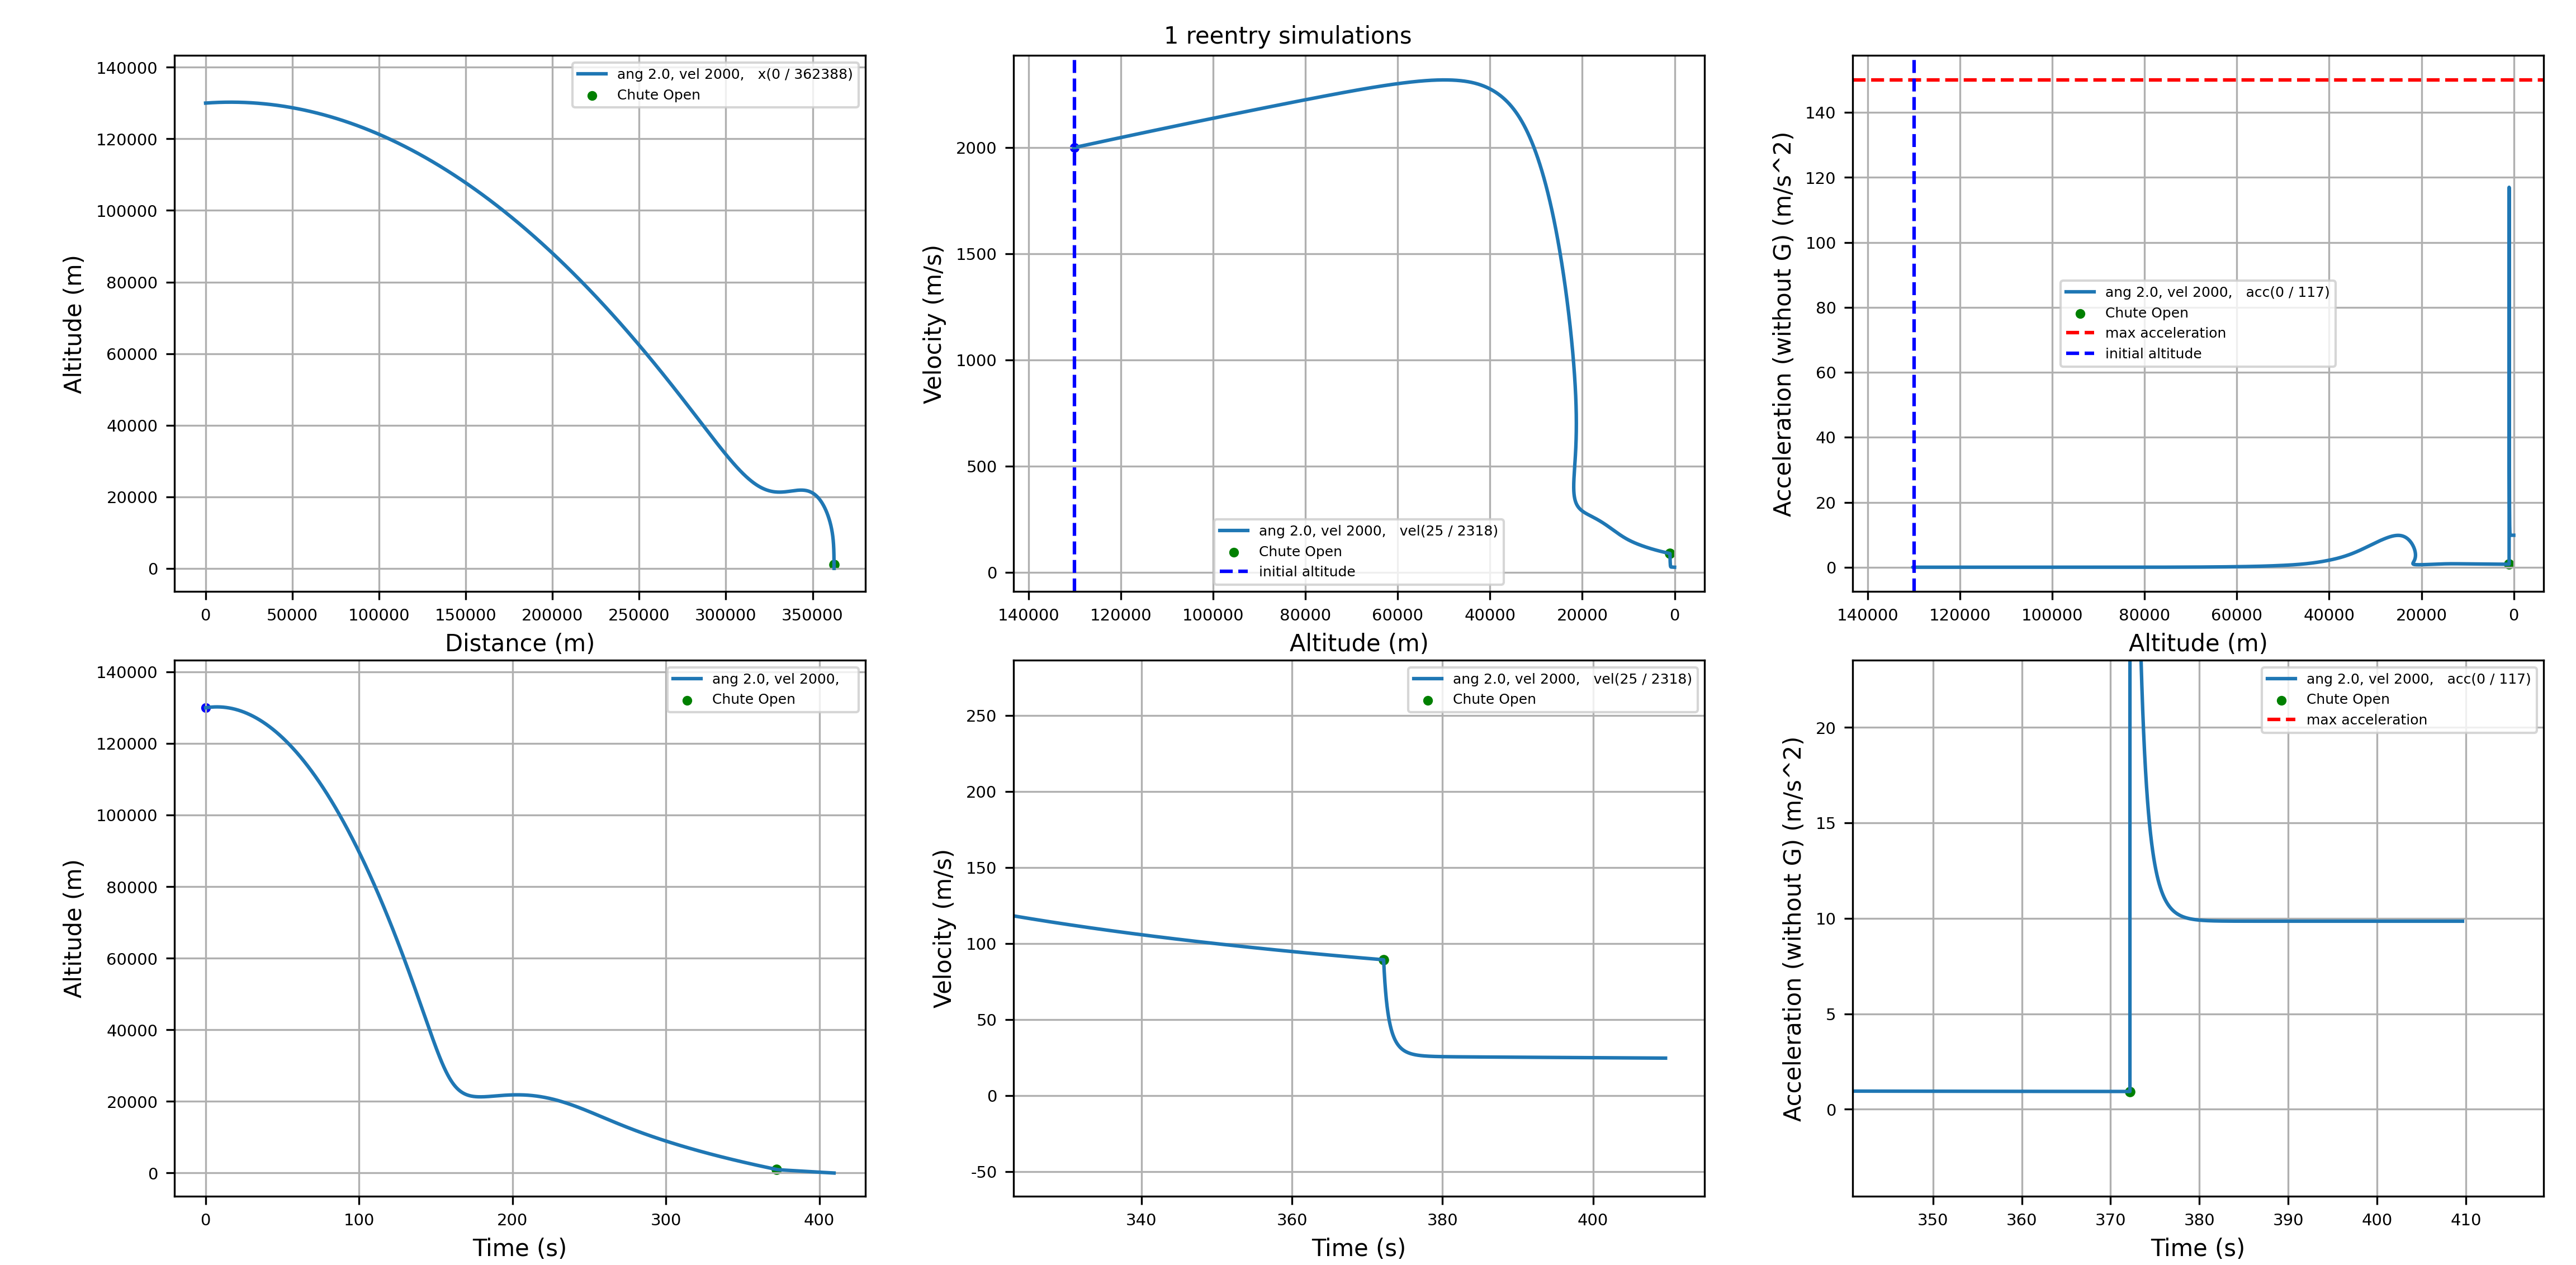
\includegraphics[width=1\textwidth]{images/forces_equilibrium_metrics.png}
\caption{Terminal Velocity} \label{forces_equilibrium}
\end{figure}







\subsection{Effect of Lift and Angle of Attack}
This simulation was made for a simple capsule reentering earth only with ballistic controls. Thus, we cannot execute correction measures such as applying the desired angle of attack. Space shuttles, for example, have better controls that allow for smoother approaches, potentially enabling land-based landings without the need for parachute deployment (except for reducing horizontal velocity after touchdown) \cite{miguel_optimal_reentry_control}. Figure \ref{attack_angle_trajectories} shows these different trajectories.

\begin{figure}[ht]
    \centering
    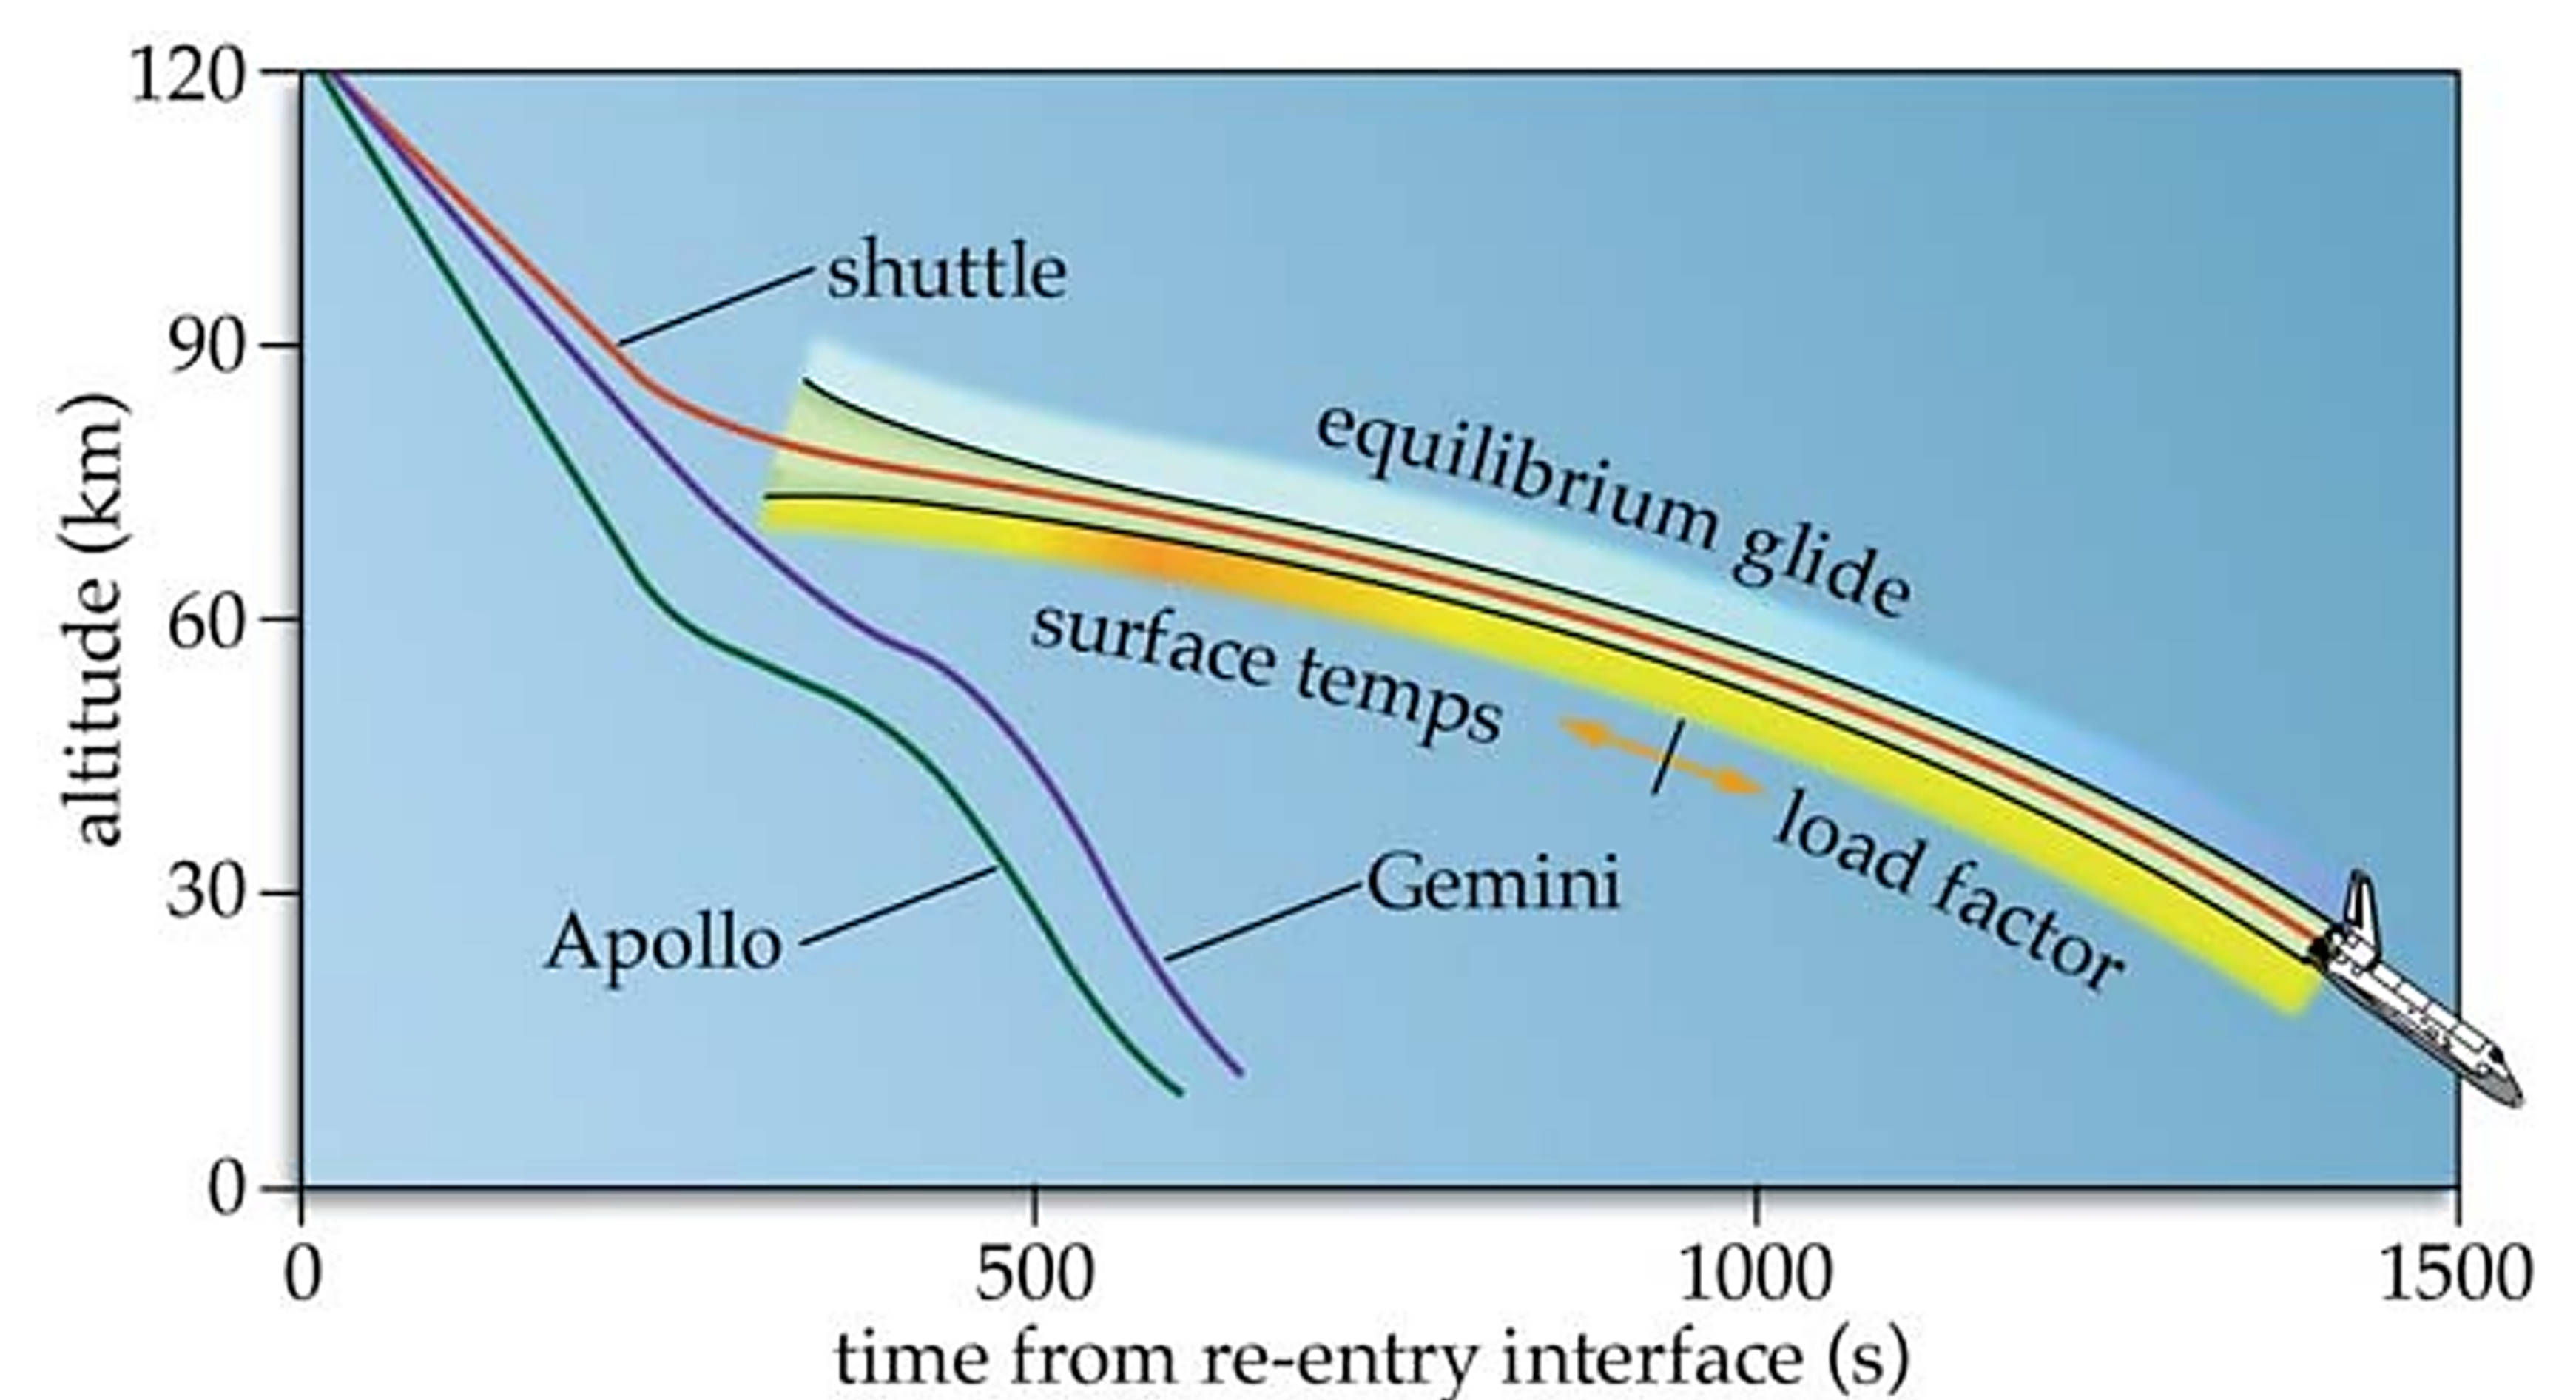
\includegraphics[width=0.75\textwidth]{images/attack_angle_trajectories.png}
    \caption{Re-entry profiles of different spacecraft \cite{returning_space}} \label{attack_angle_trajectories}
\end{figure}


For us to better understand the effects of the angle of attack on the lift, different options were implemented in the application. 

By default, lift is assumed to act perpendicular to gravity. For example, if falling vertically with no horizontal velocity, the capsule will descend vertically. However, this simplified lift force model is not realistic.

Thus, we also implemented lift to act perpendicular to velocity. We found that in this configuration, the lift force does not reduce the vertical speed as expected but instead shifts some of the velocity horizontally. For instance, when descending vertically, the lift force pushes the capsule sideways, thereby, it does not reduce the absolute speed sufficiently to allow the parachute to open.

To better understand the effects of a controlled angle of attack, a small improvement was implemented. This enhancement allows us to adjust the angle of attack of the aircraft so that the lift force pushes as vertically as possible while remaining realistic and perpendicular to the velocity vector. By setting the maximum angle of attack, we ensure that the lift vector is corrected to be as vertical as feasible. With this simulation enhancement, we can now reduce speed even during descent and enable the parachute to open.

These three scenarios are depicted in Figure \ref{lift_vs_attack_angle}: on the left, we observe lift perpendicular to gravity; in the middle, lift perpendicular to velocity without controlling the angle of attack; and on the right, lift perpendicular to velocity with corrections applied up to the specified maximum angle of attack.

\begin{figure}[ht]
    \centering
    
\includegraphics[width=1\textwidth]{images/lift_vs_attack_angle.png}
    \caption{Effect of Angle of Attack and Lift Orientation} \label{lift_vs_attack_angle}
\end{figure}






\subsection{Mission Success}
In this simulation, with the reentry interface set at an altitude of 130,000 m, and the parachutes being deployed if the altitude is 1000 m or less and the speed is 100 m/s or less, a successful reentry must ensure that the vessel and crew do not experience more than 15g (150 m/s\(^{-2}\)), that the space module touches the ocean surface at no more than 25 m/s, and that the horizontal distance projected on the Earth's surface falls between 2500 km and 4500 km. 

As inferred from the previously discussed differences between the flat Earth and round Earth models, the analysis of success criteria will lead to different outcomes. Fig. \ref{success_flat_earth} illustrates the combinations of angles and velocities required to ensure a successful landing. Additionally, Fig. \ref{sim_results_sample} depicts a sample of reentry profiles with angles ranging from 1 to 12 degrees and velocities from 8000 to 12000 m/s. This visualization aids in better understanding the trajectories, velocities, and accelerations during the reentry process.

\begin{figure}
\centering
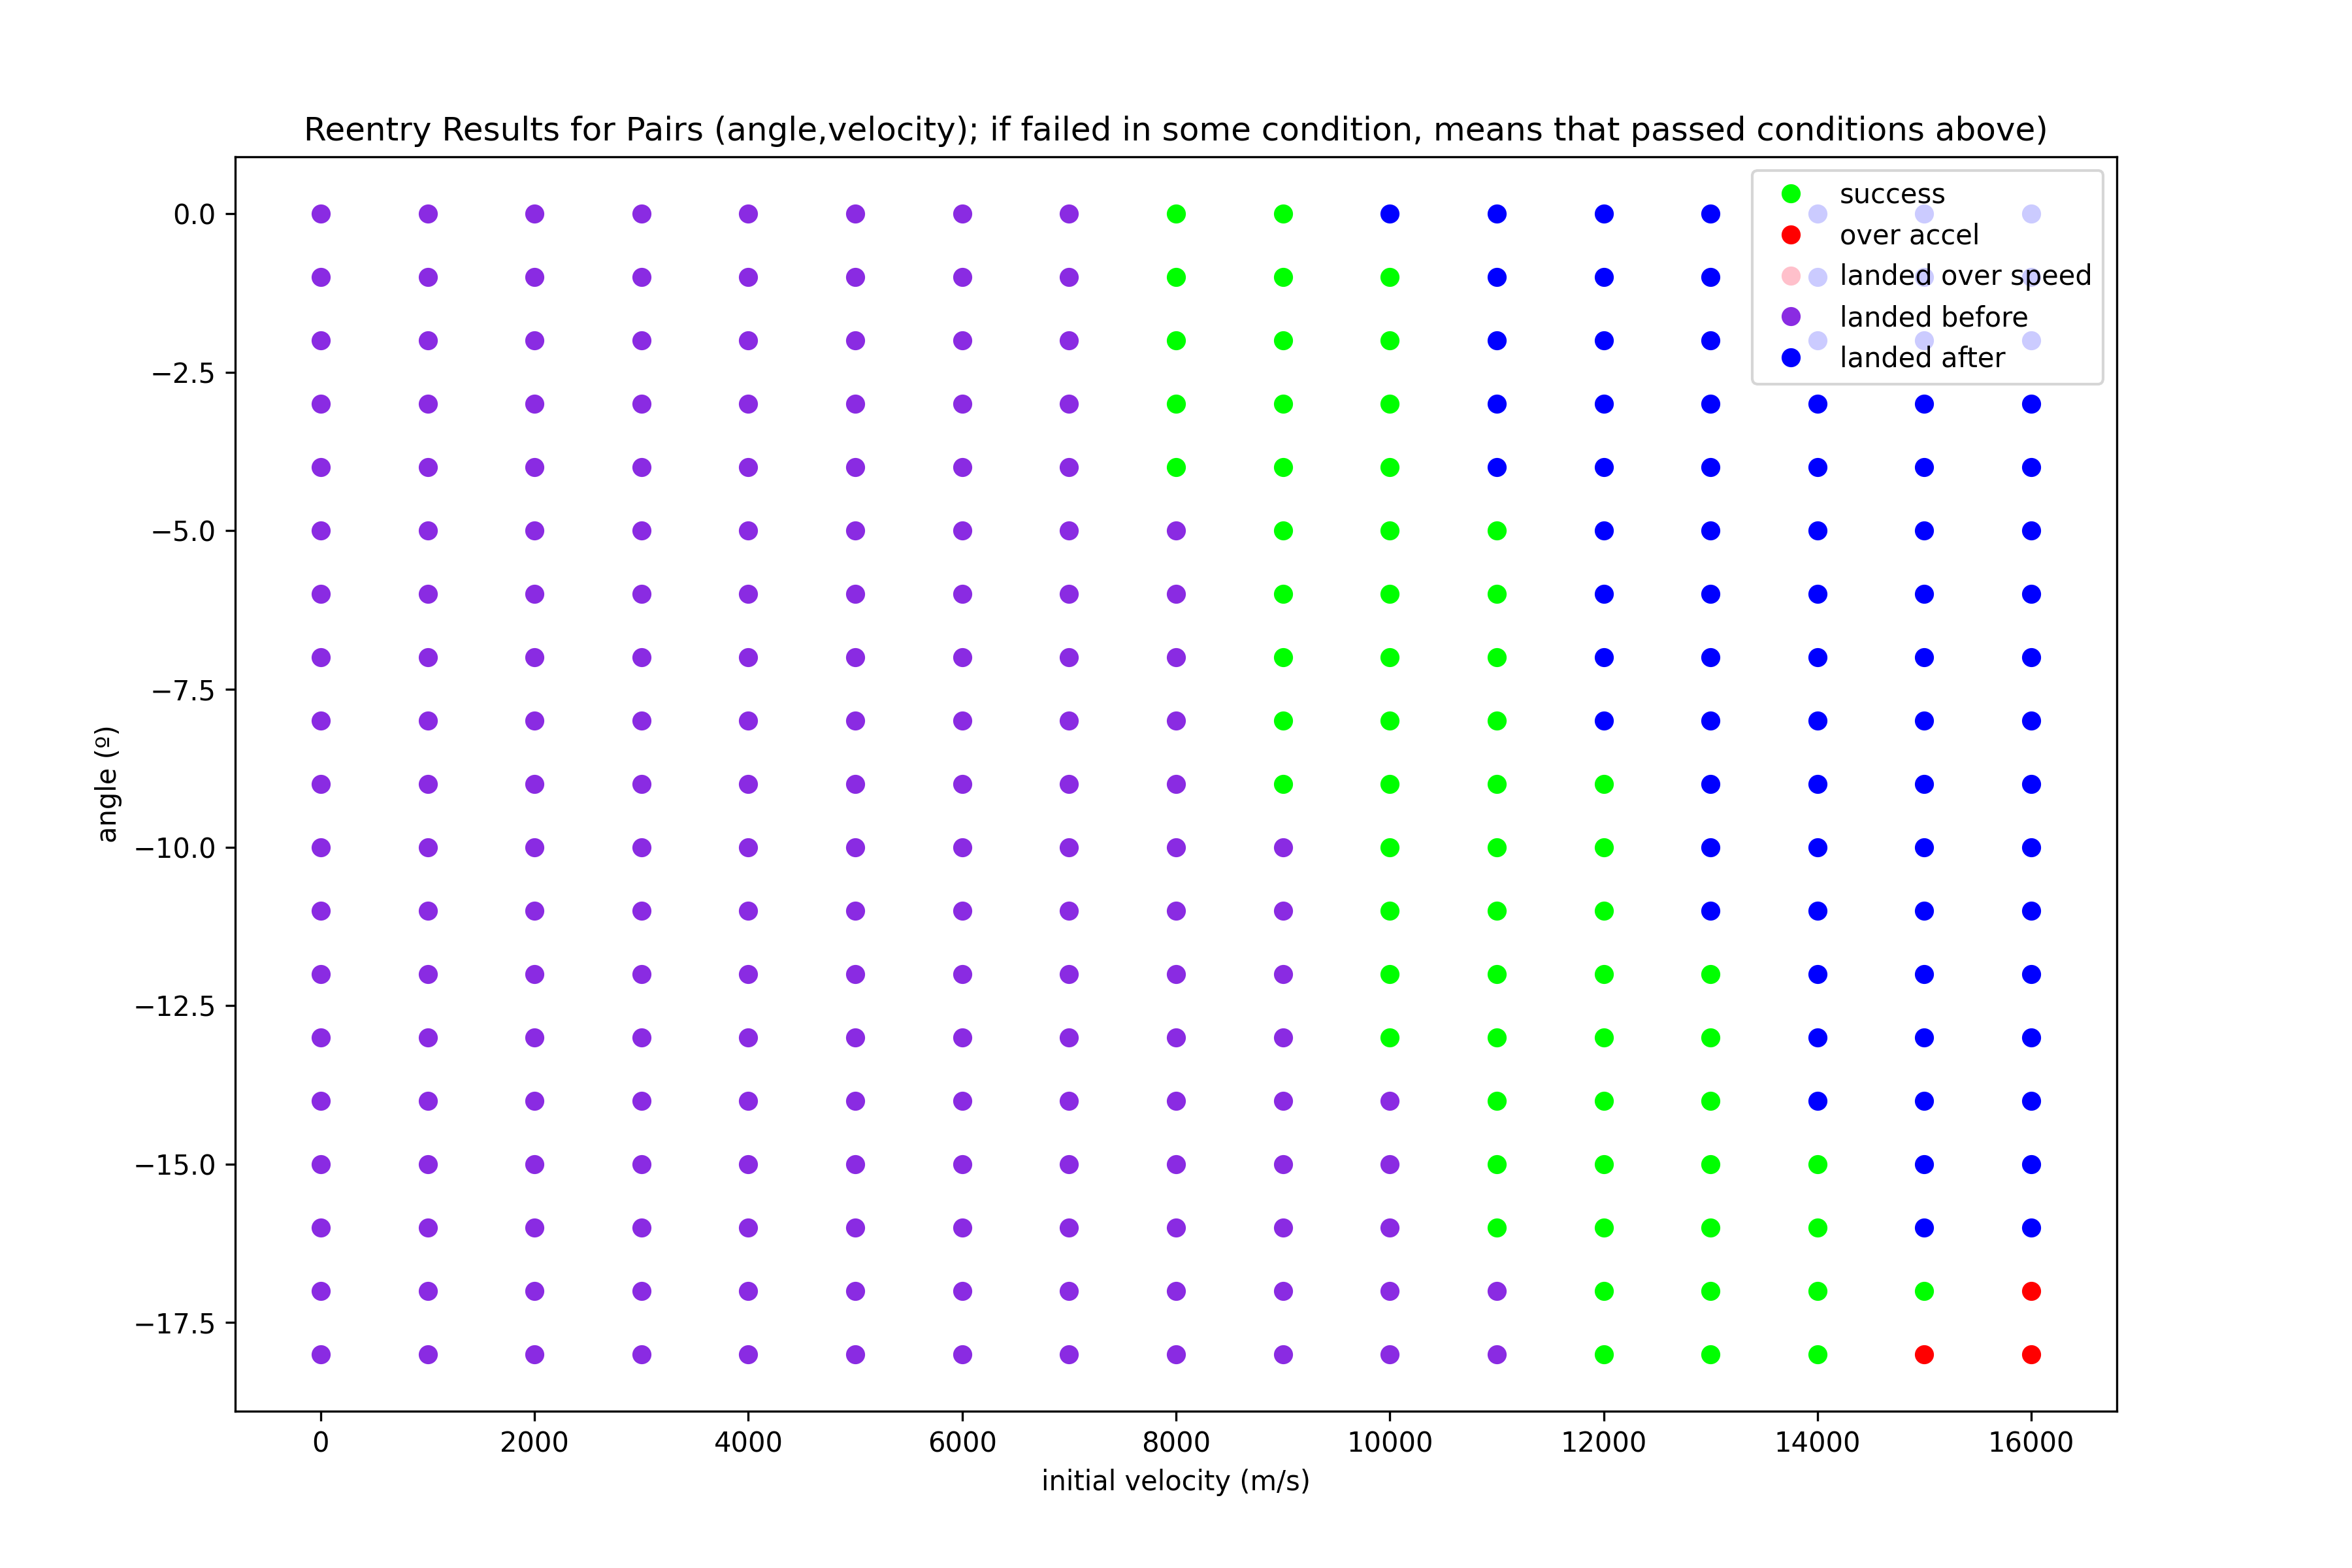
\includegraphics[width=1\textwidth]{images/success_flat_earth.png}
\caption{Mission Success on \textbf{Flat Earth} model} \label{success_flat_earth}
\end{figure}

\begin{figure}
\centering
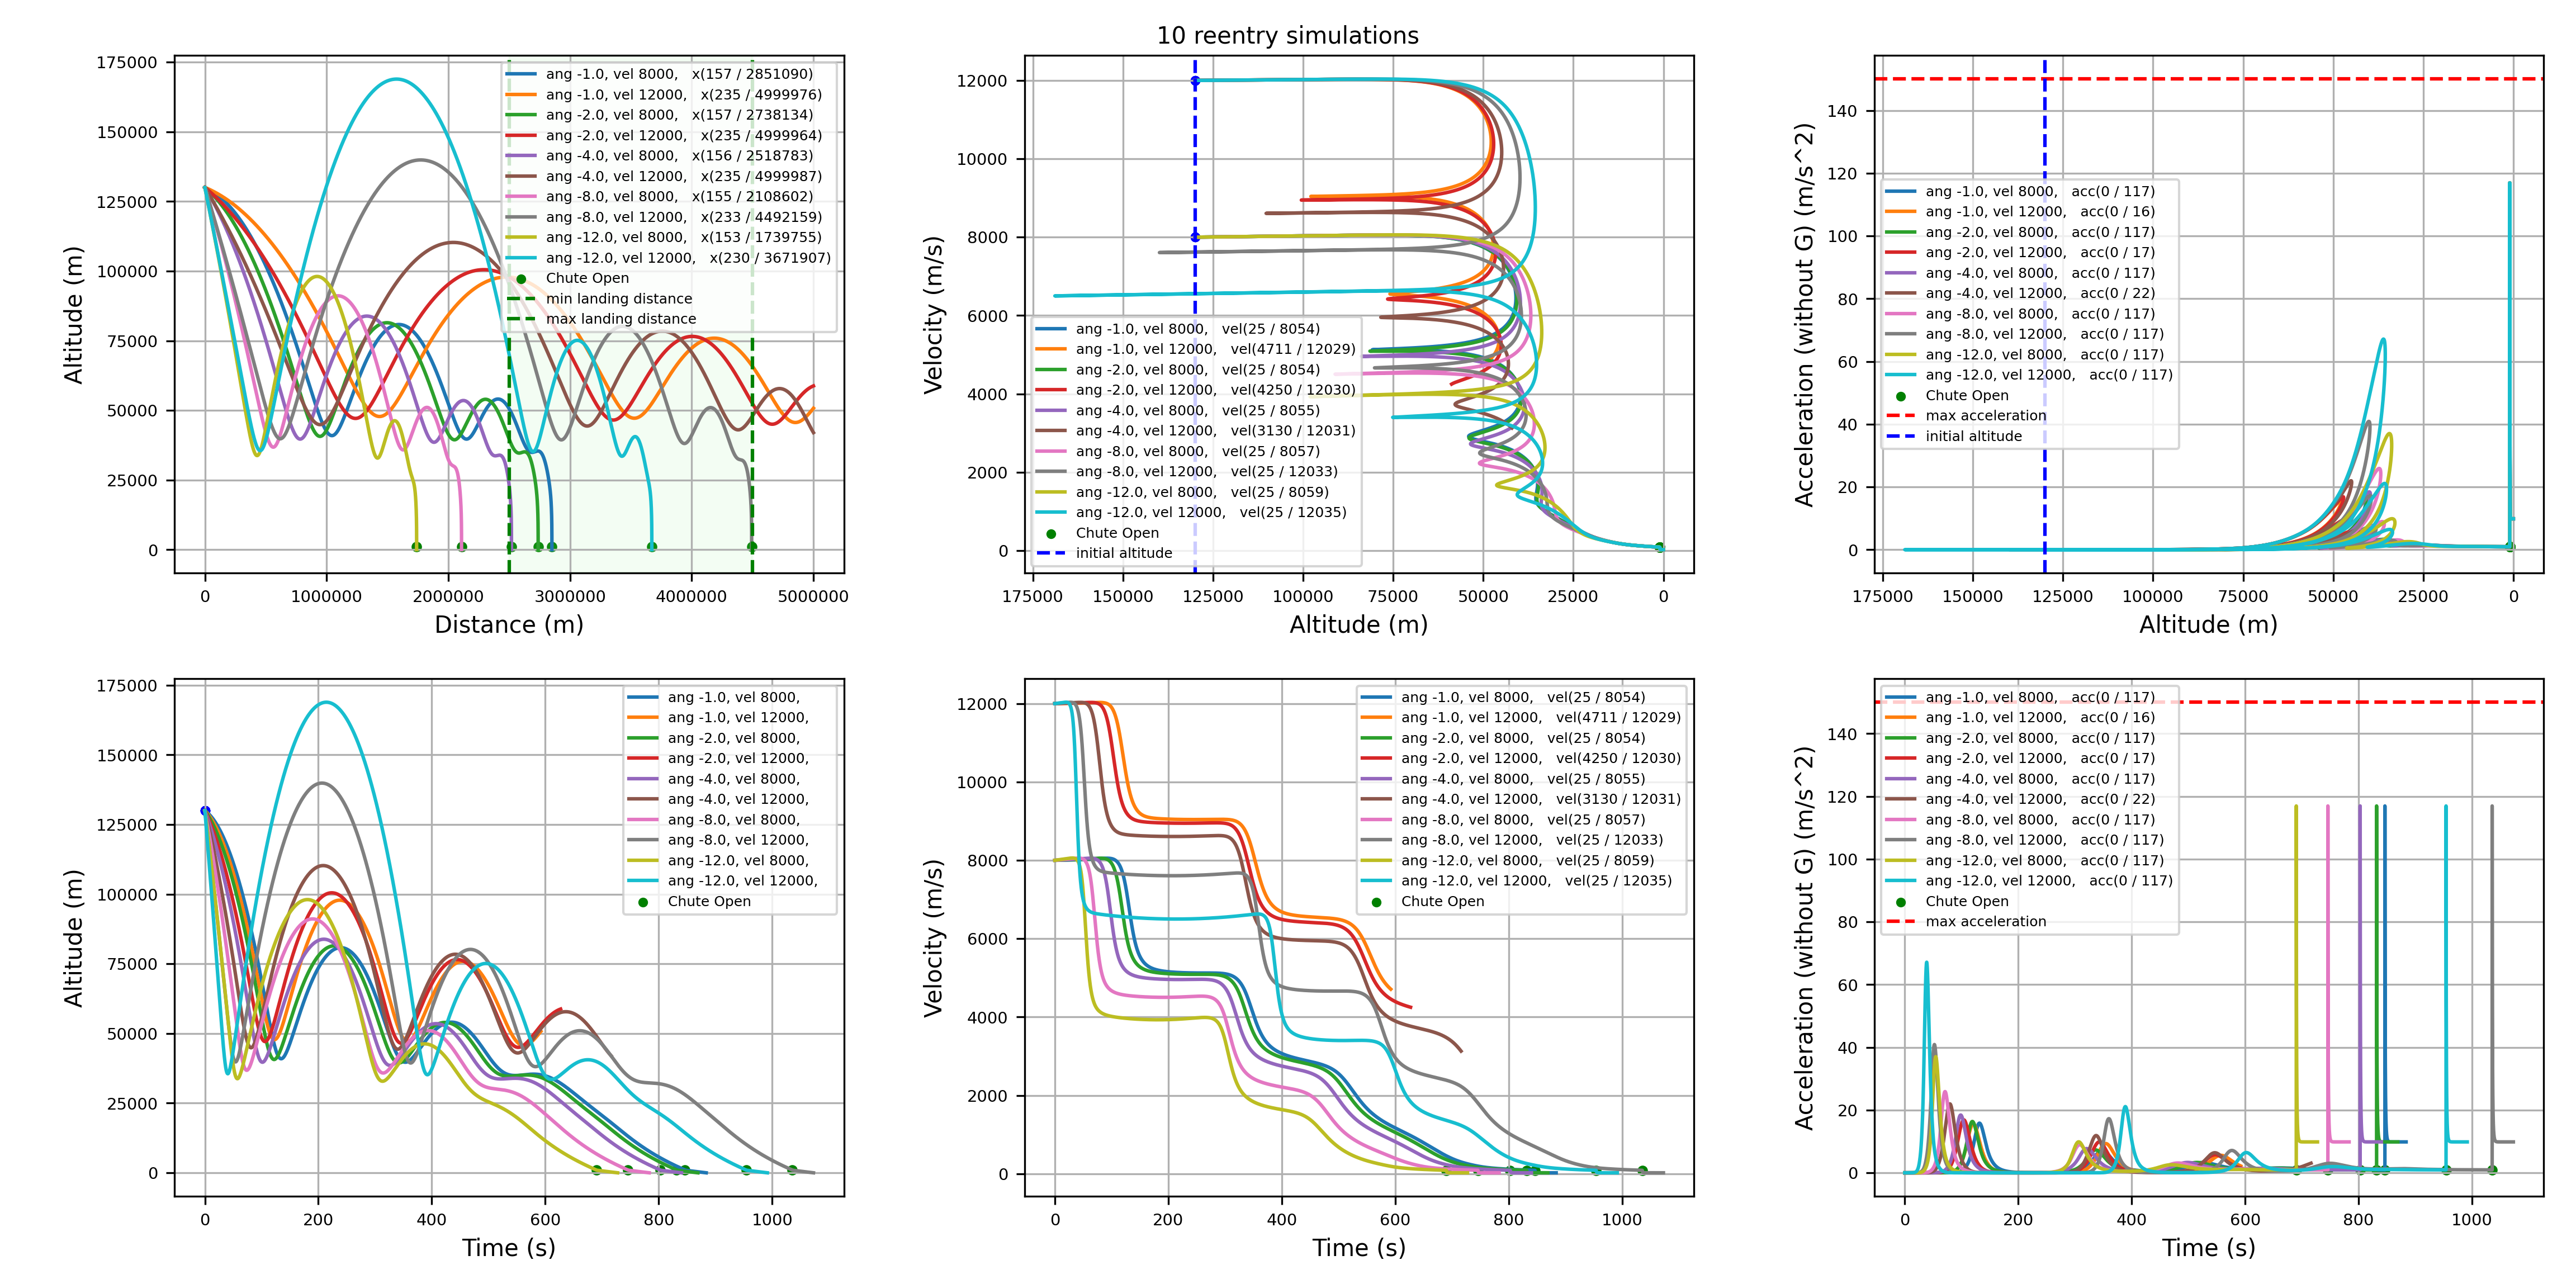
\includegraphics[width=1\textwidth]{images/sim_results_sample.png}
\caption{Re-Entry profiles for specific initial angles and velocities} \label{sim_results_sample}
\end{figure}

As observable in Fig. \ref{success_flat_earth} and Fig. \ref{sim_results_sample}, to ensure a successful re-entry, it is crucial to identify optimal combinations of entry angle and velocity. In general, a steep entry angle (close to vertical) results in a trajectory falling short of the desired landing zone. A shallow entry angle (close to horizontal) exceeds the landing zone boundaries. Very low velocities result in a vertical descent regardless of the angle (for instance, entering with zero velocity leads to a straight vertical drop). High velocities cause bouncing in the atmosphere and extend the trajectory beyond acceptable limits.
Thus, to achieve a balanced approach, velocities ranging between 7,000 and 14,000 m/s, coupled with entry angles between 1 and 15 degrees, ensure a trajectory that meets the necessary re-entry criteria without compromising safety or mission objectives\footnote{Not considering other important factors such as maximum temperature on the capsule surface, which can significantly impact the structural integrity and safety of the spacecraft.}.






%%%%%%%%%%%%%%%%%%%%%%%%%%%%%%%%%%%%%%%%%%%%%%%%%
%%%%               CONCLUSIONS               %%%%
%%%%%%%%%%%%%%%%%%%%%%%%%%%%%%%%%%%%%%%%%%%%%%%%%

\section{Conclusions}

% Key findings and contributions
We presented an application with various implementations for simulating reentry, utilizing both forward and backward methods. Our application also offers a wide range of options, allowing users to tailor the simulations to their specific goals. These options include enabling or disabling certain forces during reentry, selecting different initial angles and velocities, disabling the parachute, and simulating reentry for a round Earth. Although these options add complexity to the simulation and its implementation, they significantly enhance the application's value by providing a highly customizable and enriched user experience.

By offering these features, our application serves as a powerful tool for exploring and understanding the dynamics of reentry trajectories. Whether for educational purposes, research, or practical applications, this flexibility allows users to simulate a variety of scenarios and gain deeper insights into the factors influencing successful reentry. This adaptability ensures that our application is not only a robust educational resource but also a versatile platform for ongoing exploration and innovation in the field of aerospace dynamics.


\subsubsection*{Limitations}

Regarding simulations with a round earth model, further testing is required for edge cases, such as crossing the equator or reaching points 90 degrees away from it. The adjustments made in these scenarios need validation, as the model exhibits instability and occasionally produces overflow values in random tests.

The solver\_ivp library presents challenges in accessing and modifying values within the system during iterations, limiting manipulations primarily to the Y array, which encapsulates the system of ordinary differential equations (ODEs). Although the model functions correctly overall, the retrieval of information like acceleration or accumulated earth angle is notably harder to achieve. 


\subsubsection*{Future Works}

Upon assessing potential enhancements, it is clear that implicit methods demonstrate considerably longer runtimes in comparison to explicit methods during testing. This result is expected due to their focus on accuracy and stability. To mitigate these challenges, techniques such as multiprocessing could be utilized. This strategy allows for the simultaneous execution of multiple simulations, taking advantage of the computational power of multi-core processors.





%%%%%%%%%%%%%%%%%%%%%%%%%%%%%%%%%%%%%%%%%%%%%%%%%
%%%%               BIBLIOGRAPHY              %%%%
%%%%%%%%%%%%%%%%%%%%%%%%%%%%%%%%%%%%%%%%%%%%%%%%%

\begin{thebibliography}{10}
% Write references in style 'splncs04'
% in URLs check for  _   and put \ before (and when copying the URL to open in browser, copy it from the compiled doc and not from here with the \ bars

\bibitem{git}
F. M. S. Silva, ``farosilva0/SMCEF-P2,'' GitHub, 2024. [Online]. Available: \url{https://github.com/farosilva0/SMCEF-P2}. Accessed: Jul. 09, 2024.

\bibitem{orlando_trajectory}
J. Orlando et al., “TRAJECTORY AND ATTITUDE MODELING AND PROPAGATION FOR REENTRY DEBRIS WITH FRAGMENTATION IMPLEMENTING VOXELS MESHS.” Available: \url{http://mtc-m21c.sid.inpe.br/col/sid.inpe.br/mtc-m21c/2018/05.02.13.07/doc/publicacao.pdf}. Accessed: Jul. 02, 2024.

\bibitem{gallais_mechanics}
P. Gallais, Atmospheric Re-Entry Vehicle Mechanics. Berlin: Springer, 2007.

 \bibitem{chapman_analysis}
D. Chapman, “AN ANALYSIS OF THE CORRIDOR AND GUIDANCE REQUIREMENTS FOR SUPERCIRCULAR ENTRY INTO PLANETARY ATMOSPHERES.” Accessed: Jul. 02, 2024. [Online]. Available: \url{https://ntrs.nasa.gov/api/citations/20040030504/downloads/20040030504.pdf}.

 \bibitem{orlando_voxels}
J. Orlando et al., “TRAJECTORY AND ATTITUDE MODELING AND PROPAGATION FOR REENTRY DEBRIS WITH FRAGMENTATION IMPLEMENTING VOXELS MESHS.” Accessed: Jul. 02, 2024. [Online]. Available: \url{http://mtc-m21c.sid.inpe.br/col/sid.inpe.br/mtc-m21c/2018/05.02.13.07/doc/publicacao.pdf}.

 \bibitem{miguel_optimal_reentry_control}
A. Miguel and P. Moreira, “Optimal and Robust Control of Atmospheric Reentry Trajectories (Versão corrigida após defesa).” Available: \url{https://ubibliorum.ubi.pt/bitstream/10400.6/13015/1/8802\_19157.pdf}. Accessed: Jul. 02, 2024.


 \bibitem{reentry_matters}
“Re-Entry Matters: Investigation into Apollo Command Module Returns | AULIS Online – Different Thinking,” Aulis.com, 2014. \url{https://www.aulis.com/re-entrymatters.htm}. Accessed: Jul. 09, 2024.


 \bibitem{air_dens_site}
Editor Engineeringtoolbox, “U.S. Standard Atmosphere vs. Altitude,” Engineeringtoolbox.com, Jan. 26, 2003. \url{https://www.engineeringtoolbox.com/standard-atmosphere-d\_604.html}. Accessed: Jul. 09, 2024.
‌
\bibitem{cubic_spline}
S. McKinley and M. Levine, “Cubic Spline Interpolation.” Available: \url{https://www.rajgunesh.com/resources/downloads/numerical/cubicsplineinterpol.pdf}.

‌
 \bibitem{mazyku_optimum_reentry}
A. Mazyku and H. Blunton, "Optimum Earth Re-entry Corridors." Accessed: Jul. 10, 2024. [Online]. Available: \url{https://ntrs.nasa.gov/api/citations/19660008888/downloads/19660008888.pdf}.
‌
 \bibitem{newton_raphson_method}
“The Newton-Raphson Method.” Available: \url{https://personal.math.ubc.ca/~anstee/math104/newtonmethod.pdf}. Accessed: Jul. 10, 2024.


\bibitem{github_reentry}
“ferrolho/space-shuttle-reentry-trajectory: Space Shuttle Reentry Trajectory,” GitHub, 2024. \url{https://github.com/ferrolho/space-shuttle-reentry-trajectory}. Accessed: Jul. 02, 2024.


\end{thebibliography}


\end{document}
